\documentclass[11pt]{article}

\usepackage[a4paper]{geometry}
\geometry{left=2.0cm,right=2.0cm,top=2.5cm,bottom=2.5cm}

\usepackage{ctex} % 支持中文的LaTeX宏包
\usepackage{amsmath,amsfonts,graphicx,subfigure,amssymb,bm,amsthm,mathrsfs,mathtools,breqn} % 数学公式和符号的宏包集合
\usepackage{algorithm,algorithmicx} % 算法和伪代码的宏包
\usepackage[noend]{algpseudocode} % 算法和伪代码的宏包
\usepackage{fancyhdr} % 自定义页眉页脚的宏包
\usepackage[framemethod=TikZ]{mdframed} % 创建带边框的框架的宏包
\usepackage{fontspec} % 字体设置的宏包
\usepackage{adjustbox} % 调整盒子大小的宏包
\usepackage{fontsize} % 设置字体大小的宏包
\usepackage{tikz} % 绘制图形和使用颜色的宏包
\usepackage{pgfplots} % 绘制数据图表的宏包
\pgfplotsset{compat=1.17} % 设置pgfplots版本兼容性
\usetikzlibrary{arrows.meta,positioning} % TikZ箭头库和定位库
\usepackage{float} % 支持[H]浮动体位置参数
\usepackage{multicol} % 多栏排版的宏包
\usepackage{multirow} % 表格中合并单元格的宏包
\usepackage{pdfpages} % 插入PDF文件的宏包
\RequirePackage{listings} % 在文档中插入源代码的宏包
\usepackage{wrapfig} % 文字绕排图片的宏包
\usepackage{bigstrut,multirow,rotating} % 支持在表格中使用特殊命令的宏包
\usepackage{booktabs} % 创建美观的表格的宏包
\usepackage{threeparttable} % 支持表格注释的宏包
\usepackage{circuitikz} % 绘制电路图的宏包
\usepackage{hyperref} % 创建超链接的宏包
\usepackage[inline]{enumitem} % 自定义列表格式的宏包，支持行内列表

\definecolor{dkgreen}{rgb}{0,0.6,0}
\definecolor{gray}{rgb}{0.5,0.5,0.5}
\definecolor{mauve}{rgb}{0.58,0,0.82}
\lstset{
  frame=tb,
  aboveskip=3mm,
  belowskip=3mm,
  showstringspaces=false,
  columns=flexible,
  framerule=1pt,
  rulecolor=\color{gray!35},
  backgroundcolor=\color{gray!5},
  basicstyle={\small\ttfamily},
  numbers=none,
  numberstyle=\tiny\color{gray},
  keywordstyle=\color{blue},
  commentstyle=\color{dkgreen},
  stringstyle=\color{mauve},
  breaklines=true,
  breakatwhitespace=true,
  tabsize=3,
}


\usepackage[capitalize]{cleveref}
\Crefname{section}{Section}{Sections}
\Crefname{table}{Table}{Tables}
\crefname{table}{Table.}{Tabs.}

\setmainfont{Palatino Linotype}
\setCJKmainfont{SimSun}[BoldFont=SimHei, ItalicFont=KaiTi]
\setCJKsansfont{SimHei}
\setCJKmonofont{FangSong}
\punctstyle{kaiming}
% 偏好的几个字体, 可以根据需要自行加入字体ttf文件并调用

% Restore standard emphasis to avoid requiring an undefined environment (kaishu).
% The original redefinition used an environment `kaishu` which is not defined
% in a default ctex setup and causes compilation errors. Use \textit for
% emphasis which works across engines.
\renewcommand{\emph}[1]{\textit{#1}}

%改这里可以修改实验报告表头的信息
\newcommand{\experiName}{虚拟仪器}
\newcommand{\supervisor}{石澔玙}
\newcommand{\name}{邓思豪}
\newcommand{\studentNum}{2023K8009909008}
\newcommand{\class}{3}
\newcommand{\group}{01}
\newcommand{\seat}{5}
\newcommand{\dateYear}{2025}
\newcommand{\dateMonth}{11}
\newcommand{\dateDay}{19}
\newcommand{\room}{西实206}
\newcommand{\others}{$\square$}


\begin{document}



\begin{center}
    \LARGE \bf 《\, 基\, 础\, 物\, 理\, 实\, 验\, 》\, 实\, 验\, 报\, 告
\end{center}

\begin{center}
    \noindent \emph{实验名称}\underline{\makebox[25em][c]{\experiName}}
    \emph{指导教师}\underline{\makebox[8em][c]{\supervisor}}\\
    \emph{姓名}\underline{\makebox[6em][c]{\name}} 
    % 如果名字比较长, 可以修改box的长度"6em"
    \emph{学号}\underline{\makebox[10em][c]{\studentNum}}
    \emph{分班分组及座号} \underline{\makebox[5em][c]{\class \ -\ \group \ -\ \seat }\emph{号}} （\emph{例}:\, 1\,-\,04\,-\,5\emph{号}）\\
    \emph{实验日期} \underline{\makebox[3em][c]{\dateYear}}\emph{年}
    \underline{\makebox[2em][c]{\dateMonth}}\emph{月}
    \underline{\makebox[2em][c]{\dateDay}}\emph{日}
    \emph{实验地点}\underline{\makebox[6em][c]{\room}}
    \emph{调课/补课} \underline{\makebox[3em][c]{\others\ 是}}
    \emph{成绩评定} \underline{\hspace{5em}}
    {\noindent}
    \rule[8pt]{17cm}{0.2em}
\end{center}

\section{实验目的}
本实验旨在通过理论学习与实践操作相结合，掌握虚拟仪器相关技术及应用，具体实验目的如下：
\begin{itemize}
    \item 理解虚拟仪器的核心概念，明确其与传统仪器的本质区别及“软件就是仪器”的技术理念；
    \item 认识图形化编程语言LabVIEW的开发环境，学习该语言的基本编程逻辑与操作方法，能够独立完成简单虚拟仪器程序的搭建；
    \item 基于虚拟仪器技术，设计并实现伏安法测电阻的实验系统，完成待测电阻的测量任务，深化对虚拟仪器硬件（如NI ELVIS）与软件协同工作原理的理解。
\end{itemize}

\section{实验仪器与用具}
本实验所需仪器、用具及软件均需满足特定型号或版本要求，具体清单如下：
\begin{itemize}
    \item 计算机：含操作系统（无特定型号要求，需兼容后续软件及硬件驱动）；
    \item 虚拟仪器硬件平台：美国国家仪器公司（National Instruments）教学实验室虚拟仪器套件II\texttt{+}（NI ELVIS II\texttt{+}）及配套原型板；
    \item 软件开发平台：LabVIEW 2014（32位版本）；
    \item 连接与元件类：
          \begin{itemize}
              \item 导线：若干（用于电路连接）；
              \item 元件盒：1个，内含：100Ω标准电阻1个、1kΩ待测电阻1个、51Ω待测电阻1个、稳压二极管1个（无特定型号要求）；
              \item 温度传感器：热电偶1个（无特定型号要求，用于温度测量实验）。
          \end{itemize}
\end{itemize}

\section{实验原理}
\subsection{虚拟仪器的硬件}
本实验以计算机为基础，搭配美国国家仪器公司（National Instruments）的教学实验室虚拟仪器套件II\texttt{+}（NI ELVIS II\texttt{+}）及配套原型板作为核心硬件平台。其主要特点如下：
\begin{itemize}
    \item \textbf{NI ELVIS II\texttt{+}功能：} 集成8路差分输入（或16路单端输入）模拟数据采集通道、24路数字I/O通道，并内置示波器、数字万用表、函数发生器、二线电流电压分析仪等常用仪器功能，可通过USB与计算机连接实现数据交互。
    \item \textbf{编程与采集性能：} 支持LabVIEW定制与编程，核心模拟采集指标包括16位分辨率、单通道最高1.25 MS/s采样率，输入范围覆盖±0.1 V至±10 V，满足实验中信号采集与输出需求。
    \item \textbf{原型板：} 为外部元件（如电阻、二极管）提供接线接口与电源支持。
\end{itemize}

\subsection{虚拟仪器的软件}
本实验采用LabVIEW 2014（32位）作为虚拟仪器开发平台。LabVIEW是图形化编程语言，其编制的程序称为虚拟仪器（VI），每个VI包含三个核心部分：
\begin{itemize}
    \item \textbf{前面板（Front Panel）：} 模拟真实仪器面板，包含输入控件（如旋钮、开关）与显示控件（如数值显示、图表），用于参数设置与结果展示；
    \item \textbf{程序框图（Block Diagram）：} 对应仪器内部功能逻辑，由端口（传递数据）、节点（调用函数/子程序）、图框（控制程序结构）及连线（传递数据流）组成；
    \item \textbf{图标/连线板：} 用于VI的调用与数据交互。
\end{itemize}
LabVIEW遵循数据流编程模式，仅当模块输入数据完全就绪时才执行，执行后将数据传递至后续模块，确保程序逻辑有序运行。

\subsection{虚拟仪器测量伏安特性原理}
本实验通过虚拟仪器实现伏安法测电阻，核心原理如下：
\begin{enumerate}
    \item \textbf{供电与采集方案：} 利用NI ELVIS II\texttt{+}的1路模拟输出通道为测量电路提供电压，2路模拟输入通道分别采集电路总电压（$U_{\text{总}}$）与标准电阻（$R_{\text{标}}$）两端电压（$U_{\text{标}}$）。
    \item \textbf{数据计算：} 根据欧姆定律，电路电流$I = \frac{U_{\text{标}}}{R_{\text{标}}}$，待测电阻两端电压$U_{\text{待}} = U_{\text{总}} - U_{\text{标}}$。
    \item \textbf{电阻求解：} 程序控制模拟输出电压从0 V逐步增至设定值，每改变一次电压采集一组$U_{\text{待}}$与$I$数据，形成数组后通过线性拟合（以$I$为横坐标、$U_{\text{待}}$为纵坐标），拟合直线的斜率即为待测电阻值（$R_{\text{待}} = \frac{U_{\text{待}}}{I}$）。
    \item \textbf{输入方式注意事项：} 采用单端输入时，所有模拟输入通道共用地线（AIGND），连线需确保接地可靠，避免干扰。
\end{enumerate}

测量原理如图\ref{fig:fig4_voltampere_principle}所示。

\begin{figure}[htbp]
    \centering
    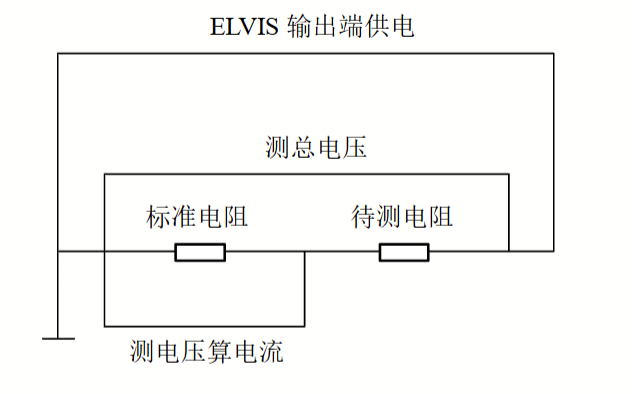
\includegraphics[width=0.6\textwidth]{fig4_voltampere_principle.png}
    \caption{用虚拟仪器测量伏安特性原理图}
    \label{fig:fig4_voltampere_principle}
\end{figure}

\section{实验内容}

\subsection{LabVIEW开发环境的启动与界面操作步骤}
本小节详细介绍LabVIEW 2014开发环境的启动流程及核心界面的操作方法：
\begin{enumerate}
    \item \textbf{程序启动}：通过计算机开始菜单路径启动LabVIEW 2014，具体步骤为："开始$\rightarrow$所有程序$\rightarrow$National Instruments$\rightarrow$LabVIEW 2014$\rightarrow$LabVIEW 2014"，执行后启动LabVIEW程序；
    \item \textbf{新建VI与界面切换}：选择"文件$\rightarrow$新建VI"进入LabVIEW开发环境，此时将显示\textbf{前面板}与\textbf{程序框图}两个核心窗口；通过"窗口$\rightarrow$显示程序框图"可从前面板切换至程序框图，同理可反向切换；
    \item \textbf{选板调用与使用}：
          \begin{itemize}
              \item 在前面板界面，点击"查看$\rightarrow$控件选板"或"查看$\rightarrow$工具选板"，可分别调出控件选板（含旋钮、开关等控制量图标）与工具选板；将控件选板中的图标放置到前面板后，对应的端子与图标会同步显示在程序框图中，实现数据的控制与结果显示（操作界面参见图\ref{fig:fig5_control_panel}）；
              \item 在程序框图窗口，点击"查看$\rightarrow$函数选板"调出函数选板，利用其提供的循环、数学运算、比较等函数功能，可搭建框图程序；
          \end{itemize}
    \item \textbf{基础操作熟悉}：尝试熟悉各选板上的图标与名称，练习选择并放置控件、右键查看快捷菜单，掌握标签工具、定位工具、连线工具的使用方法，同时熟悉各类快捷键（详细操作说明可参考软件附录）。
\end{enumerate}

\begin{figure}[htbp]
    \centering
    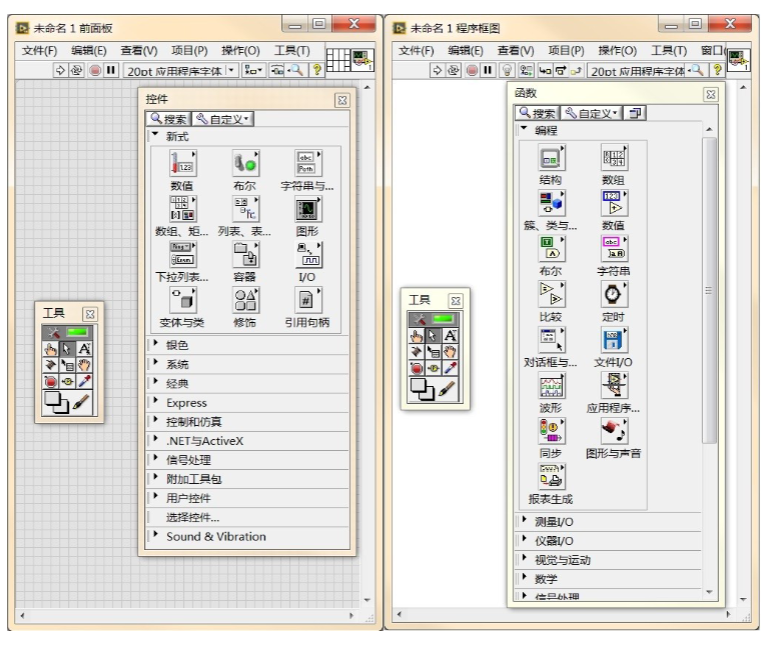
\includegraphics[width=0.7\textwidth]{fig5_control_panel.png}
    \caption{LabVIEW前面板与控件选板操作界面示意图}
    \label{fig:fig5_control_panel}
\end{figure}

\subsection{模拟温度测量程序的创建}
本小节基于LabVIEW 2014实现模拟温度测量程序，利用控件模拟温度传感器的电压输出，并实现摄氏/华氏温度的切换显示，具体内容如下：

\subsubsection{温度测量的模拟原理}
仪器通过温度传感器（如热电偶）将温度（非电学量）转换为电压（热电动势，电学量）信号。本实验模拟“输出电压与温度成正比”的传感器：设定华氏温度$80^\circ\text{F}$对应传感器输出电压$0.8\ \text{V}$，程序将基于该对应关系由输入电压计算温度，并通过开关实现摄氏温度与华氏温度的显示切换。


\subsubsection{实验步骤}
\subsubsection{创建前面板}
新建空白VI并打开前面板窗口，通过控件选板添加并配置如下控件（界面示意见图\ref{fig:fig6_temp_frontpanel}）：
\begin{itemize}
    \item \textbf{温度计控件：} 路径"控件$\rightarrow$数值$\rightarrow$温度计"，用于直观显示温度；
    \item \textbf{垂直滑动杆开关：} 路径"控件$\rightarrow$布尔$\rightarrow$垂直滑动杆开关"，用标签工具将名称改为"温度值单位"；右键开关选择"显示项$\rightarrow$布尔文本"，在"条件真"旁添加标签"摄氏"，"条件假"旁添加"华氏"；
    \item \textbf{数值显示控件：} 路径"控件$\rightarrow$数值$\rightarrow$数值显示控件"，标签改为"温度值"；
    \item \textbf{数值输入控件：} 路径"控件$\rightarrow$数值$\rightarrow$数值输入控件"，标签改为"采集的电压"（用于模拟传感器输出电压）。
\end{itemize}

\begin{figure}[htbp]
    \centering
    \begin{minipage}[b]{0.45\textwidth}
        \centering
        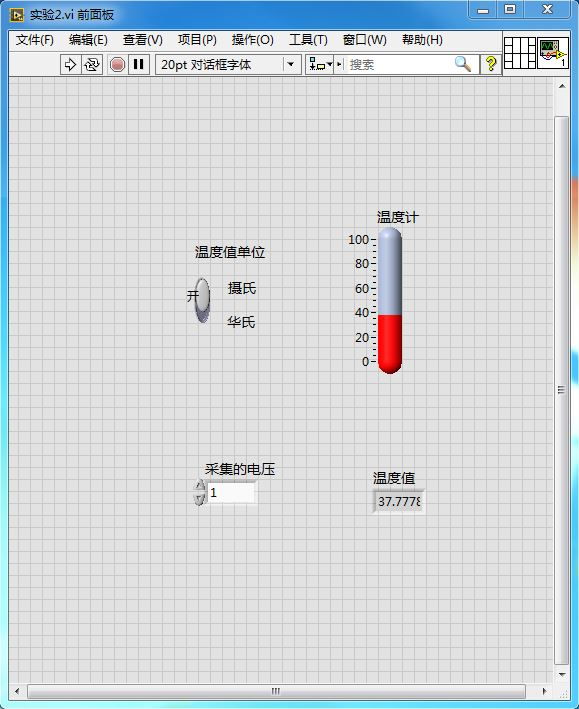
\includegraphics[width=\textwidth]{fig6_temp_frontpanel.JPG}
        \caption{模拟温度测量前面板图}
        \label{fig:fig6_temp_frontpanel}
    \end{minipage}
    \hspace{0.05\textwidth}
    \begin{minipage}[b]{0.45\textwidth}
        \centering
        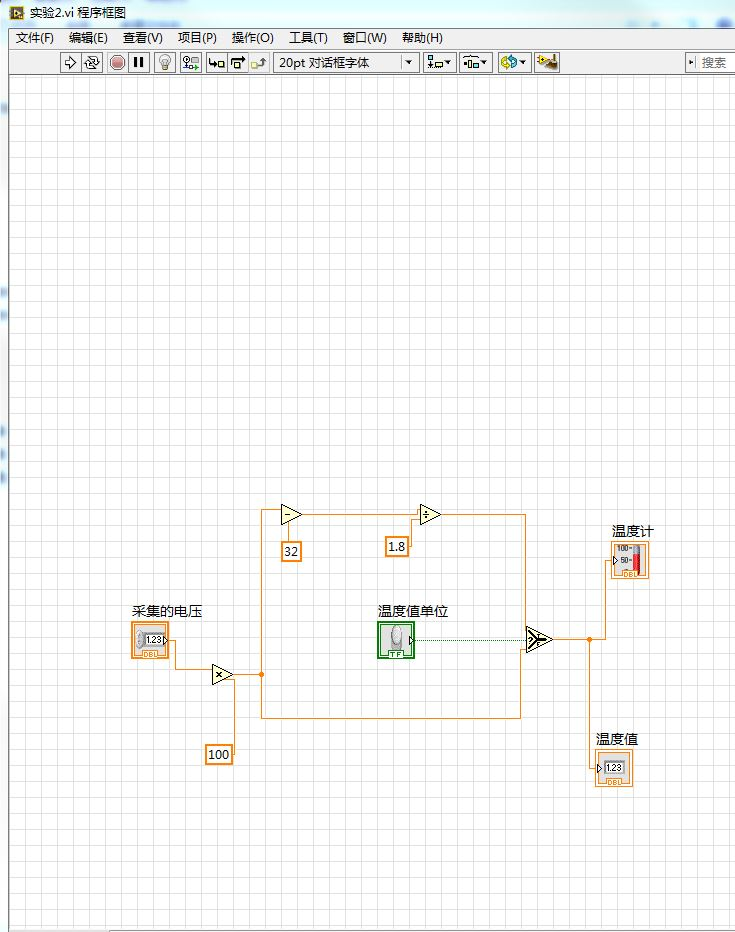
\includegraphics[width=\textwidth]{fig7_temp_blockdiagram.JPG}
        \caption{模拟温度测量程序框图}
        \label{fig:fig7_temp_blockdiagram}
    \end{minipage}
\end{figure}


\subsubsection{创建程序框图}
打开程序框图窗口，通过函数选板添加并连接如下对象（结构见图\ref{fig:fig7_temp_blockdiagram}）：
\begin{itemize}
    \item \textbf{数值运算函数：} 添加"乘法""减法""除法"函数（路径：函数$\rightarrow$数值）；
    \item \textbf{选择函数：} 添加"选择"函数（路径：函数$\rightarrow$比较），该函数含2个数值输入端（t、f）与1个布尔输入端（s）：当 s 为真时输出 t（摄氏温度），为假时输出 f（华氏温度）；
    \item \textbf{常量与连线：} 通过连线工具将各控件、函数端口连接，并创建数值常量（如 32、1.8、100），调整图标位置后整理连线（右键连线选择"整理连线"）。
\end{itemize}


\subsubsection{运行程序}
程序运行与测试步骤：
\begin{enumerate}
    \item 切换至前面板窗口，点击"连续运行"按钮，使程序进入连续运行模式；
    \item 调整"采集的电压"输入值（建议在 $0.5\sim 2$ 之间），切换"温度值单位"开关，观察"温度计"与"温度值"的显示变化，分析程序各模块的功能；
    \item 点击"连续运行"按钮停止程序，通过"文件$\rightarrow$保存"（或快捷键 Ctrl+S）保存 VI 文件。
\end{enumerate}

\subsection{电压输出与采集程序的创建}
本部分基于LabVIEW 2014与NI ELVIS硬件平台，创建电压输出与采集程序，实现模拟电压的输出及同步采集功能，其前面板与程序框图分别如图\ref{fig:fig12_voltage_frontpanel}、图\ref{fig:fig13_voltage_blockdiagram}所示。

\subsubsection{实验步骤}
\subsubsection{编写输出电压程序}
新建空白VI并在程序框图中完成如下操作：
\begin{enumerate}
    \item \textbf{创建虚拟通道：} 打开函数选板，选择"测量I/O$\rightarrow$DAQmx$\rightarrow$数据采集$\rightarrow$DAQmx创建虚拟通道"，将该图标拖入程序框图；右键图标选择"选择类型$\rightarrow$模拟输出$\rightarrow$电压"，并在弹出的"物理通道"选项处右键，选择"创建$\rightarrow$输入控件"，生成输出通道的选择控件。
    \item \textbf{添加任务节点：} 在"测量I/O$\rightarrow$DAQmx$\rightarrow$数据采集"中，依次添加"DAQmx开始任务""DAQmx写入""DAQmx清除任务"节点；在"DAQmx写入"的数据输入端右键，选择"创建$\rightarrow$输入控件"，生成输出电压的输入控件。
    \item \textbf{构建循环与控制模块：}
          \begin{itemize}
              \item 从函数选板"结构"中选择"While循环"，放置在程序框图合适位置；
              \item 从"定时"函数中添加"等待ms"，并为其创建数值常量100（即"等待100 ms"）；
              \item 在前面板"控件$\rightarrow$布尔"中添加停止按钮，将"等待100 ms"与停止按钮放入While循环内；
              \item 使用连线工具将各节点、控件的端口按逻辑连接。
          \end{itemize}
\end{enumerate}


\subsubsection{编写采集电压程序}
采用与输出电压程序类似的方法，在程序框图中创建电压采集的虚拟通道（选择"模拟输入$\rightarrow$电压"类型），添加"DAQmx开始任务""DAQmx读取""DAQmx清除任务"节点，生成测量电压的显示控件，整理各图标与连线（程序结构见图\ref{fig:fig13_voltage_blockdiagram}）。

\subsubsection{硬件连接}
打开NI ELVIS电源与原型板电源，按如下方式完成电路连线：
\begin{itemize}
    \item 用导线连接原型板的模拟输出端“AO 0”与模拟输入端“AI0 +”；
    \item 用导线连接“AI0 -”端与接地端“AIGND”。
\end{itemize}


\subsubsection{运行程序}
程序运行与测试步骤：
\begin{enumerate}
    \item 在前面板中设置通道：输出通道选择"Dev3/ao0"，输入通道选择"Dev3/ai0"；
    \item 运行VI程序，调整"输出电压"输入值，观察"测量电压"的同步变化；
    \item 点击"停止输出""停止测量"按钮，观察程序暂停情况；
    \item 停止程序运行后，通过"文件$\rightarrow$保存"（或快捷键 Ctrl+S）保存 VI 文件。
\end{enumerate}

\subsubsection{程序界面与框图}
\begin{figure}[htbp]
    \centering
    \begin{minipage}[b]{0.45\textwidth}
        \centering
        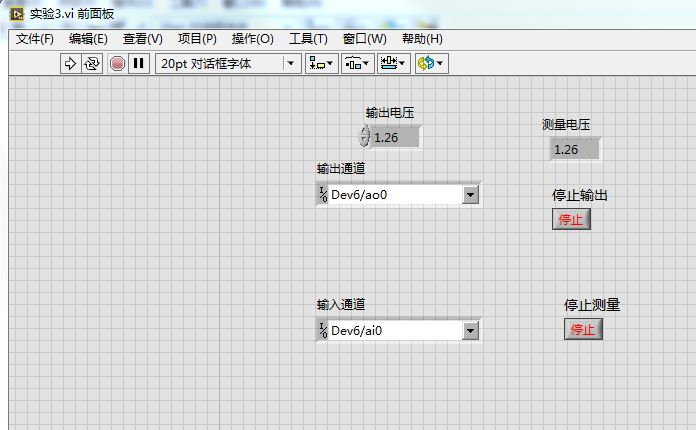
\includegraphics[width=\textwidth]{fig12_voltage_frontpanel.JPG}
        \caption{电压输出和采集前面板图}
        \label{fig:fig12_voltage_frontpanel}
    \end{minipage}
    \hspace{0.05\textwidth}
    \begin{minipage}[b]{0.45\textwidth}
        \centering
        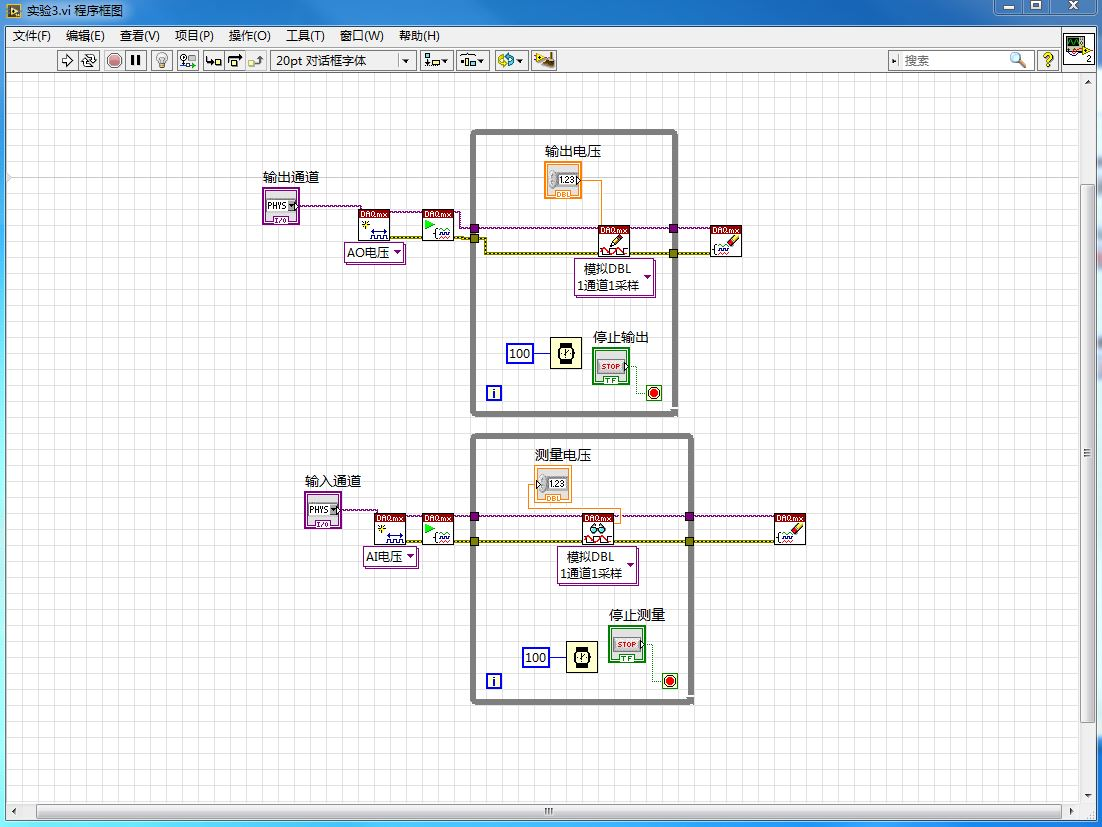
\includegraphics[width=\textwidth]{fig13_voltage_blockdiagram.JPG}
        \caption{电压输出和采集程序框图}
        \label{fig:fig13_voltage_blockdiagram}
    \end{minipage}
\end{figure}

\subsection{基于虚拟仪器的伏安特性测量程序创建与实验}
本部分通过LabVIEW 2014与NI ELVIS II+平台，创建伏安特性测量程序，实现待测电阻的伏安曲线绘制与阻值计算，其前面板与程序框图分别如图\ref{fig:fig14_voltamp_frontpanel}、图\ref{fig:fig15_voltamp_blockdiagram}所示。


\subsubsection{创建前面板}
按照以下步骤完成前面板控件的添加与配置：
\begin{enumerate}
    \item 添加伏安曲线显示控件：
          从"控件选板$\rightarrow$图形$\rightarrow$Express XY图"中添加控件，命名为"电阻的伏安曲线图"；将纵坐标改为"电流（A）"、横坐标改为"电压（V）"；在图右上角"曲线0"处右键，选择"常用曲线$\rightarrow$点+线"模式。
    \item 添加数值输入控件：
          放入4个数值型输入控件，分别命名为"输出电压步长""测量数据点数""标准电阻""时间间隔"；在"时间间隔"控件右键选择"显示项$\rightarrow$单位标签"，输入单位"s"；同理为"输出电压步长"添加单位"V"。
    \item 添加显示与控制控件：
          放入1个数值型显示控件，命名为"待测电阻值"；放入1个二维数组显示控件（路径："控件选板$\rightarrow$数组、矩阵与簇$\rightarrow$数组"，添加数值型显示控件后设为二维），命名为"数据"；放入1个开关按钮（路径："控件$\rightarrow$布尔$\rightarrow$开关按钮"），用于控制程序进程。
\end{enumerate}
配置完成的前面板如图\ref{fig:fig14_voltamp_frontpanel}所示。

\begin{figure}[htbp]
    \centering
    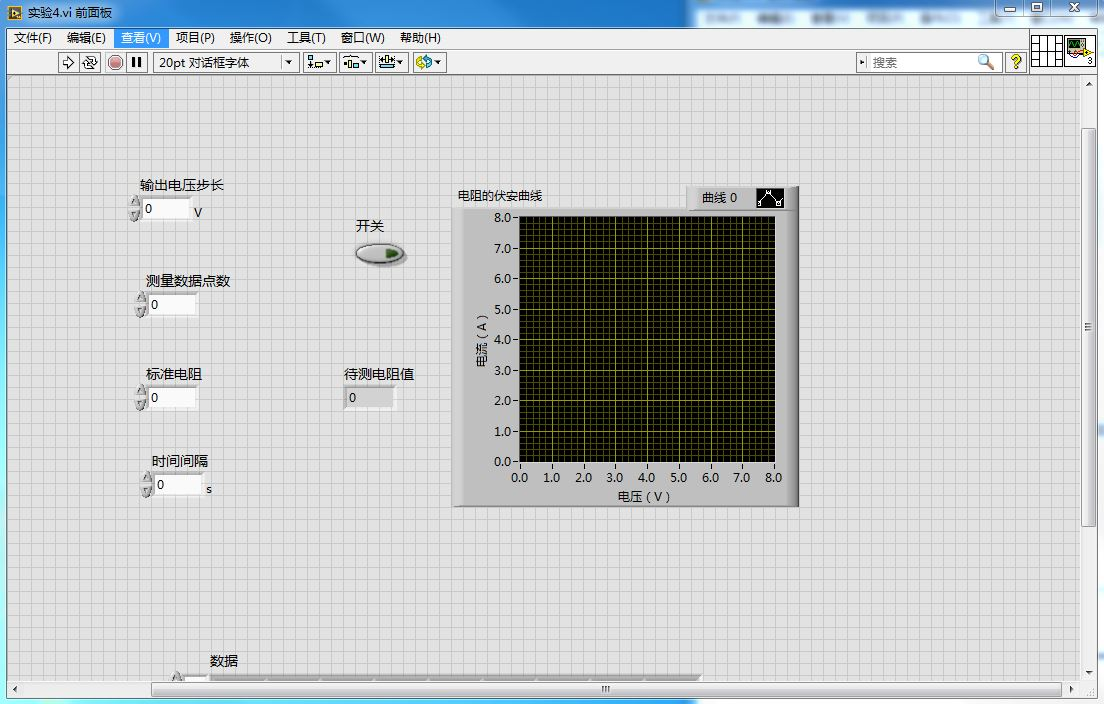
\includegraphics[width=0.7\textwidth]{fig14_voltamp_frontpanel.JPG} % 替换为实际图路径
    \caption{伏安法测电阻前面板图}
    \label{fig:fig14_voltamp_frontpanel}
\end{figure}


\subsubsection{创建程序框图}
程序框图采用“顺序结构+While循环”实现电压逐步输出与数据采集，具体步骤如下：

\paragraph{（1）搭建5帧顺序结构}
从"函数$\rightarrow$结构$\rightarrow$平铺式顺序结构"中添加控件，右键边框选择"在后面添加帧"，扩展为5帧，将各控件图标对应放入各帧：
\begin{itemize}
    \item \textbf{第0帧（电压输出）}：
          添加"DAQ助手"（路径："函数$\rightarrow$Express$\rightarrow$输出$\rightarrow$DAQ助手"），选择"生成信号$\rightarrow$模拟输出$\rightarrow$电压"，物理通道选"Dev3 (NI ELVIS II+)$\rightarrow$ao0"，生成模式设为"1采样（按要求）"。
    \item \textbf{第1帧（等待电路稳定）}：
          添加"等待（ms）"（路径："函数$\rightarrow$定时"）与"单位转换"（路径："函数$\rightarrow$数值$\rightarrow$转换"）；在"单位转换"中输入"ms"，将"时间间隔"（单位s）转换为ms后连接至"等待（ms）"输入端。
    \item \textbf{第2帧（电压采集与计算）}：
          添加"DAQ助手"（路径："函数$\rightarrow$Express$\rightarrow$采集$\rightarrow$DAQ助手"），选择"采集信号$\rightarrow$模拟输入$\rightarrow$电压"，物理通道选"Dev3$\rightarrow$ai0、ai1"，生成模式设为"1采样（按要求）"；
          添加"索引数组"（路径："函数$\rightarrow$数组"），创建索引常量0、1，分别提取总电压与标准电阻电压；
          添加"减""除"节点（路径："函数$\rightarrow$数值"），通过"总电压-标准电阻电压"得待测电阻电压，通过"标准电阻电压/标准电阻"得电路电流。
    \item \textbf{第3帧（测量后等待）}：
          添加“等待（ms）”，创建数值常量“100”（即等待100 ms），减少数据测量干扰。
    \item \textbf{第4帧（电压复位）}：
          添加“DAQ助手”，设置电压输出为0 V，使程序结束时输出复位。
\end{itemize}

\paragraph{（2）嵌套While循环实现电压步进}
\begin{enumerate}
    \item 将顺序结构、"数据""电阻的伏安曲线图"全部包含在"While循环"（路径："函数$\rightarrow$结构"）内；
    \item 实现电压步进：将循环变量$i$与"输出电压步长"相乘，连接至第0帧DAQ助手的数据端，使输出电压从0 V开始逐步递增；
    \item 设置循环条件：将循环变量$i$与"测量数据点数"比较，与开关按钮做"与"运算（路径："函数$\rightarrow$布尔$\rightarrow$与"），连接至循环条件端（设为"真时继续"）。
\end{enumerate}

\paragraph{（3）数据存储与显示}
\begin{enumerate}
    \item 添加2个移位寄存器（右键While循环边框选择"添加移位寄存器"），用于存储电压、电流数据；
    \item 添加"创建数组"（路径："函数$\rightarrow$数组"），将新测量的电压、电流与移位寄存器中的历史数据拼接为一维数组；
    \item 再添加"创建数组"，将电压数组与电流数组合并为二维数组，连接至"数据"显示控件；将电压数组、电流数组分别连接至"电阻的伏安曲线图"的X、Y输入端。
\end{enumerate}

\paragraph{（4）阻值计算}
在While循环外添加"线性拟合"节点（路径："函数$\rightarrow$数学$\rightarrow$拟合$\rightarrow$线性拟合"），将电流数组、电压数组分别连接至X、Y输入端，拟合斜率（即待测电阻值）连接至"待测电阻值"显示控件。

配置完成的程序框图如图\ref{fig:fig15_voltamp_blockdiagram}所示。

\begin{figure}[htbp]
    \centering
    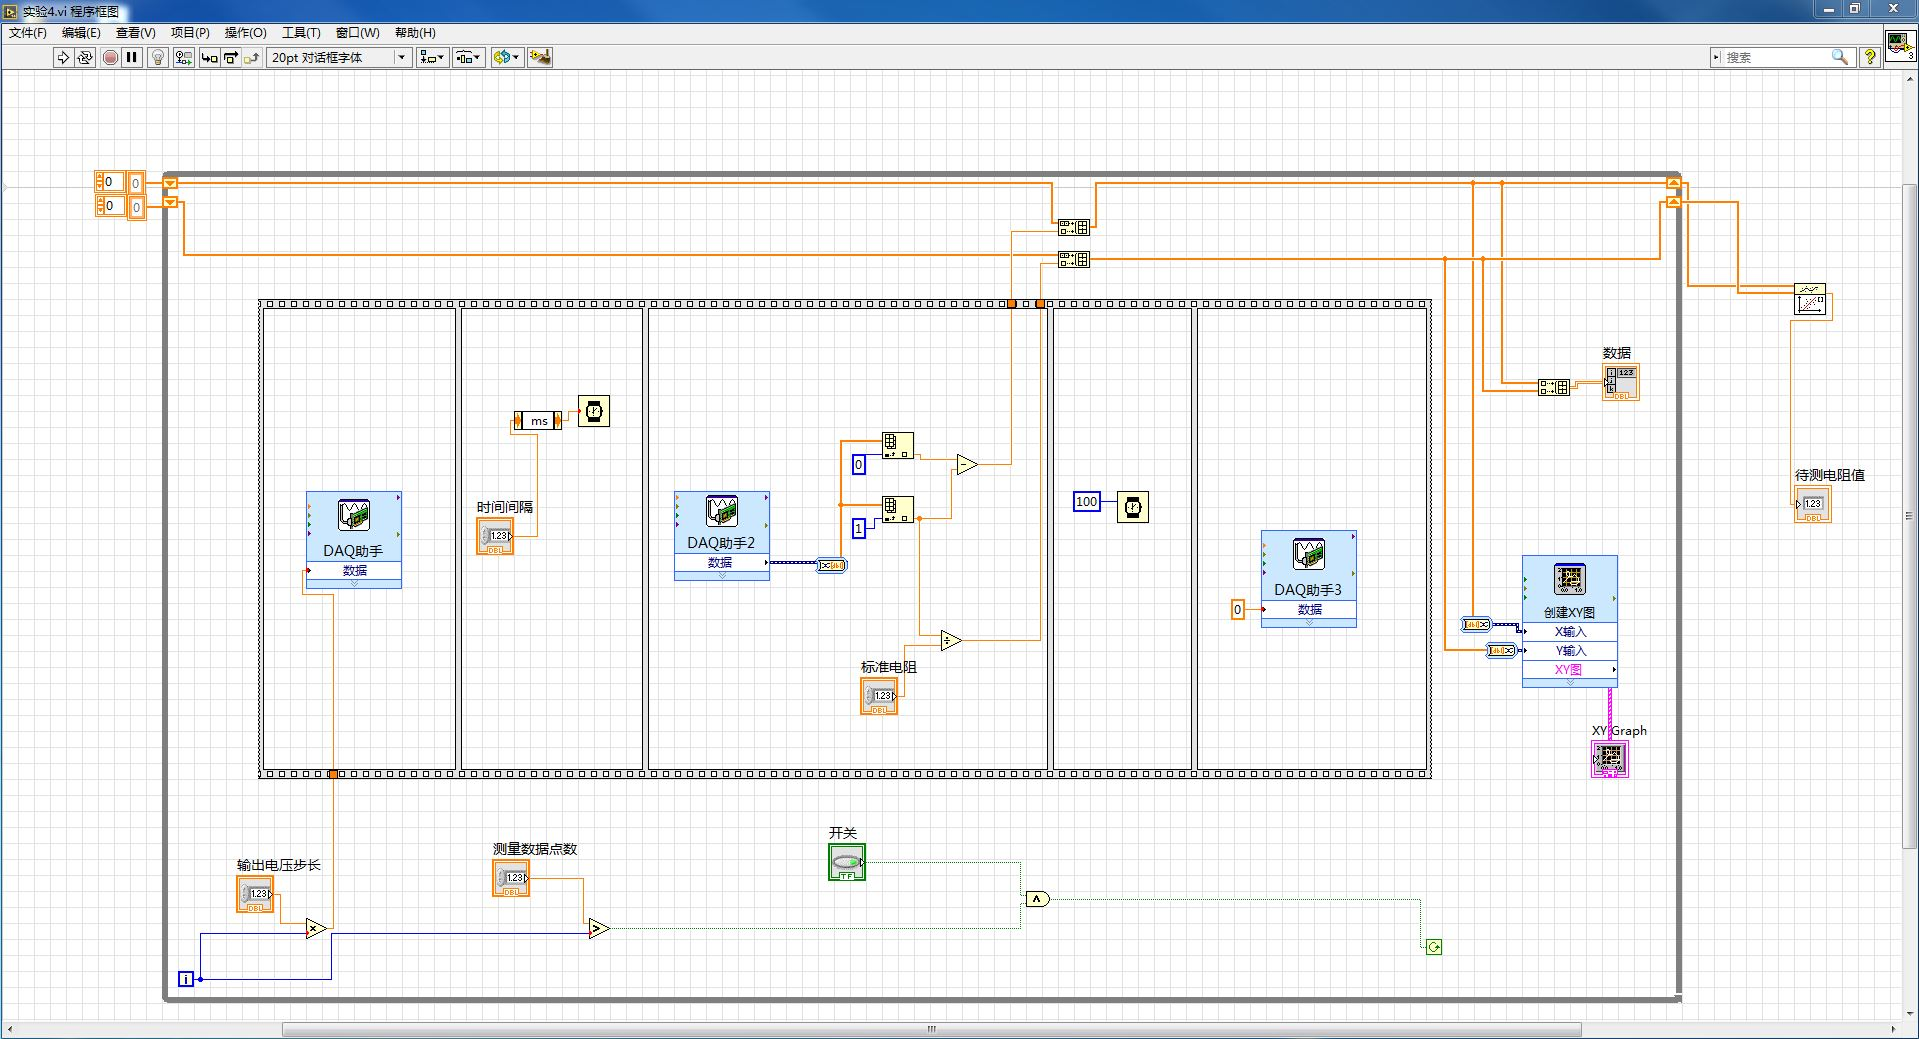
\includegraphics[width=0.8\textwidth]{fig15_voltamp_blockdiagram.JPG} % 替换为实际图路径
    \caption{伏安法测电阻程序框图}
    \label{fig:fig15_voltamp_blockdiagram}
\end{figure}


\subsubsection{正确连接外部电路}
在NI ELVIS II+原型板上完成电路连接：将模拟输出端“AO 0”接入测量电路总输入端，标准电阻与待测电阻串联后接至模拟输入端“AI0”“AI1”，公共端接原型板接地端“AIGND”。


\subsubsection{运行程序}
\begin{enumerate}
    \item 检查前面板参数设置（如输出电压步长、测量数据点数等），打开NI ELVIS电源与原型板电源；
    \item 运行VI程序，观察“电阻的伏安曲线图”与“数据”的实时更新，记录“待测电阻值”；
    \item 更换待测电阻，重复测量并分析实验结果。
\end{enumerate}

\section{实验数据与处理}

\subsection{实验电路连接}
\begin{figure}[H]
    \centering
    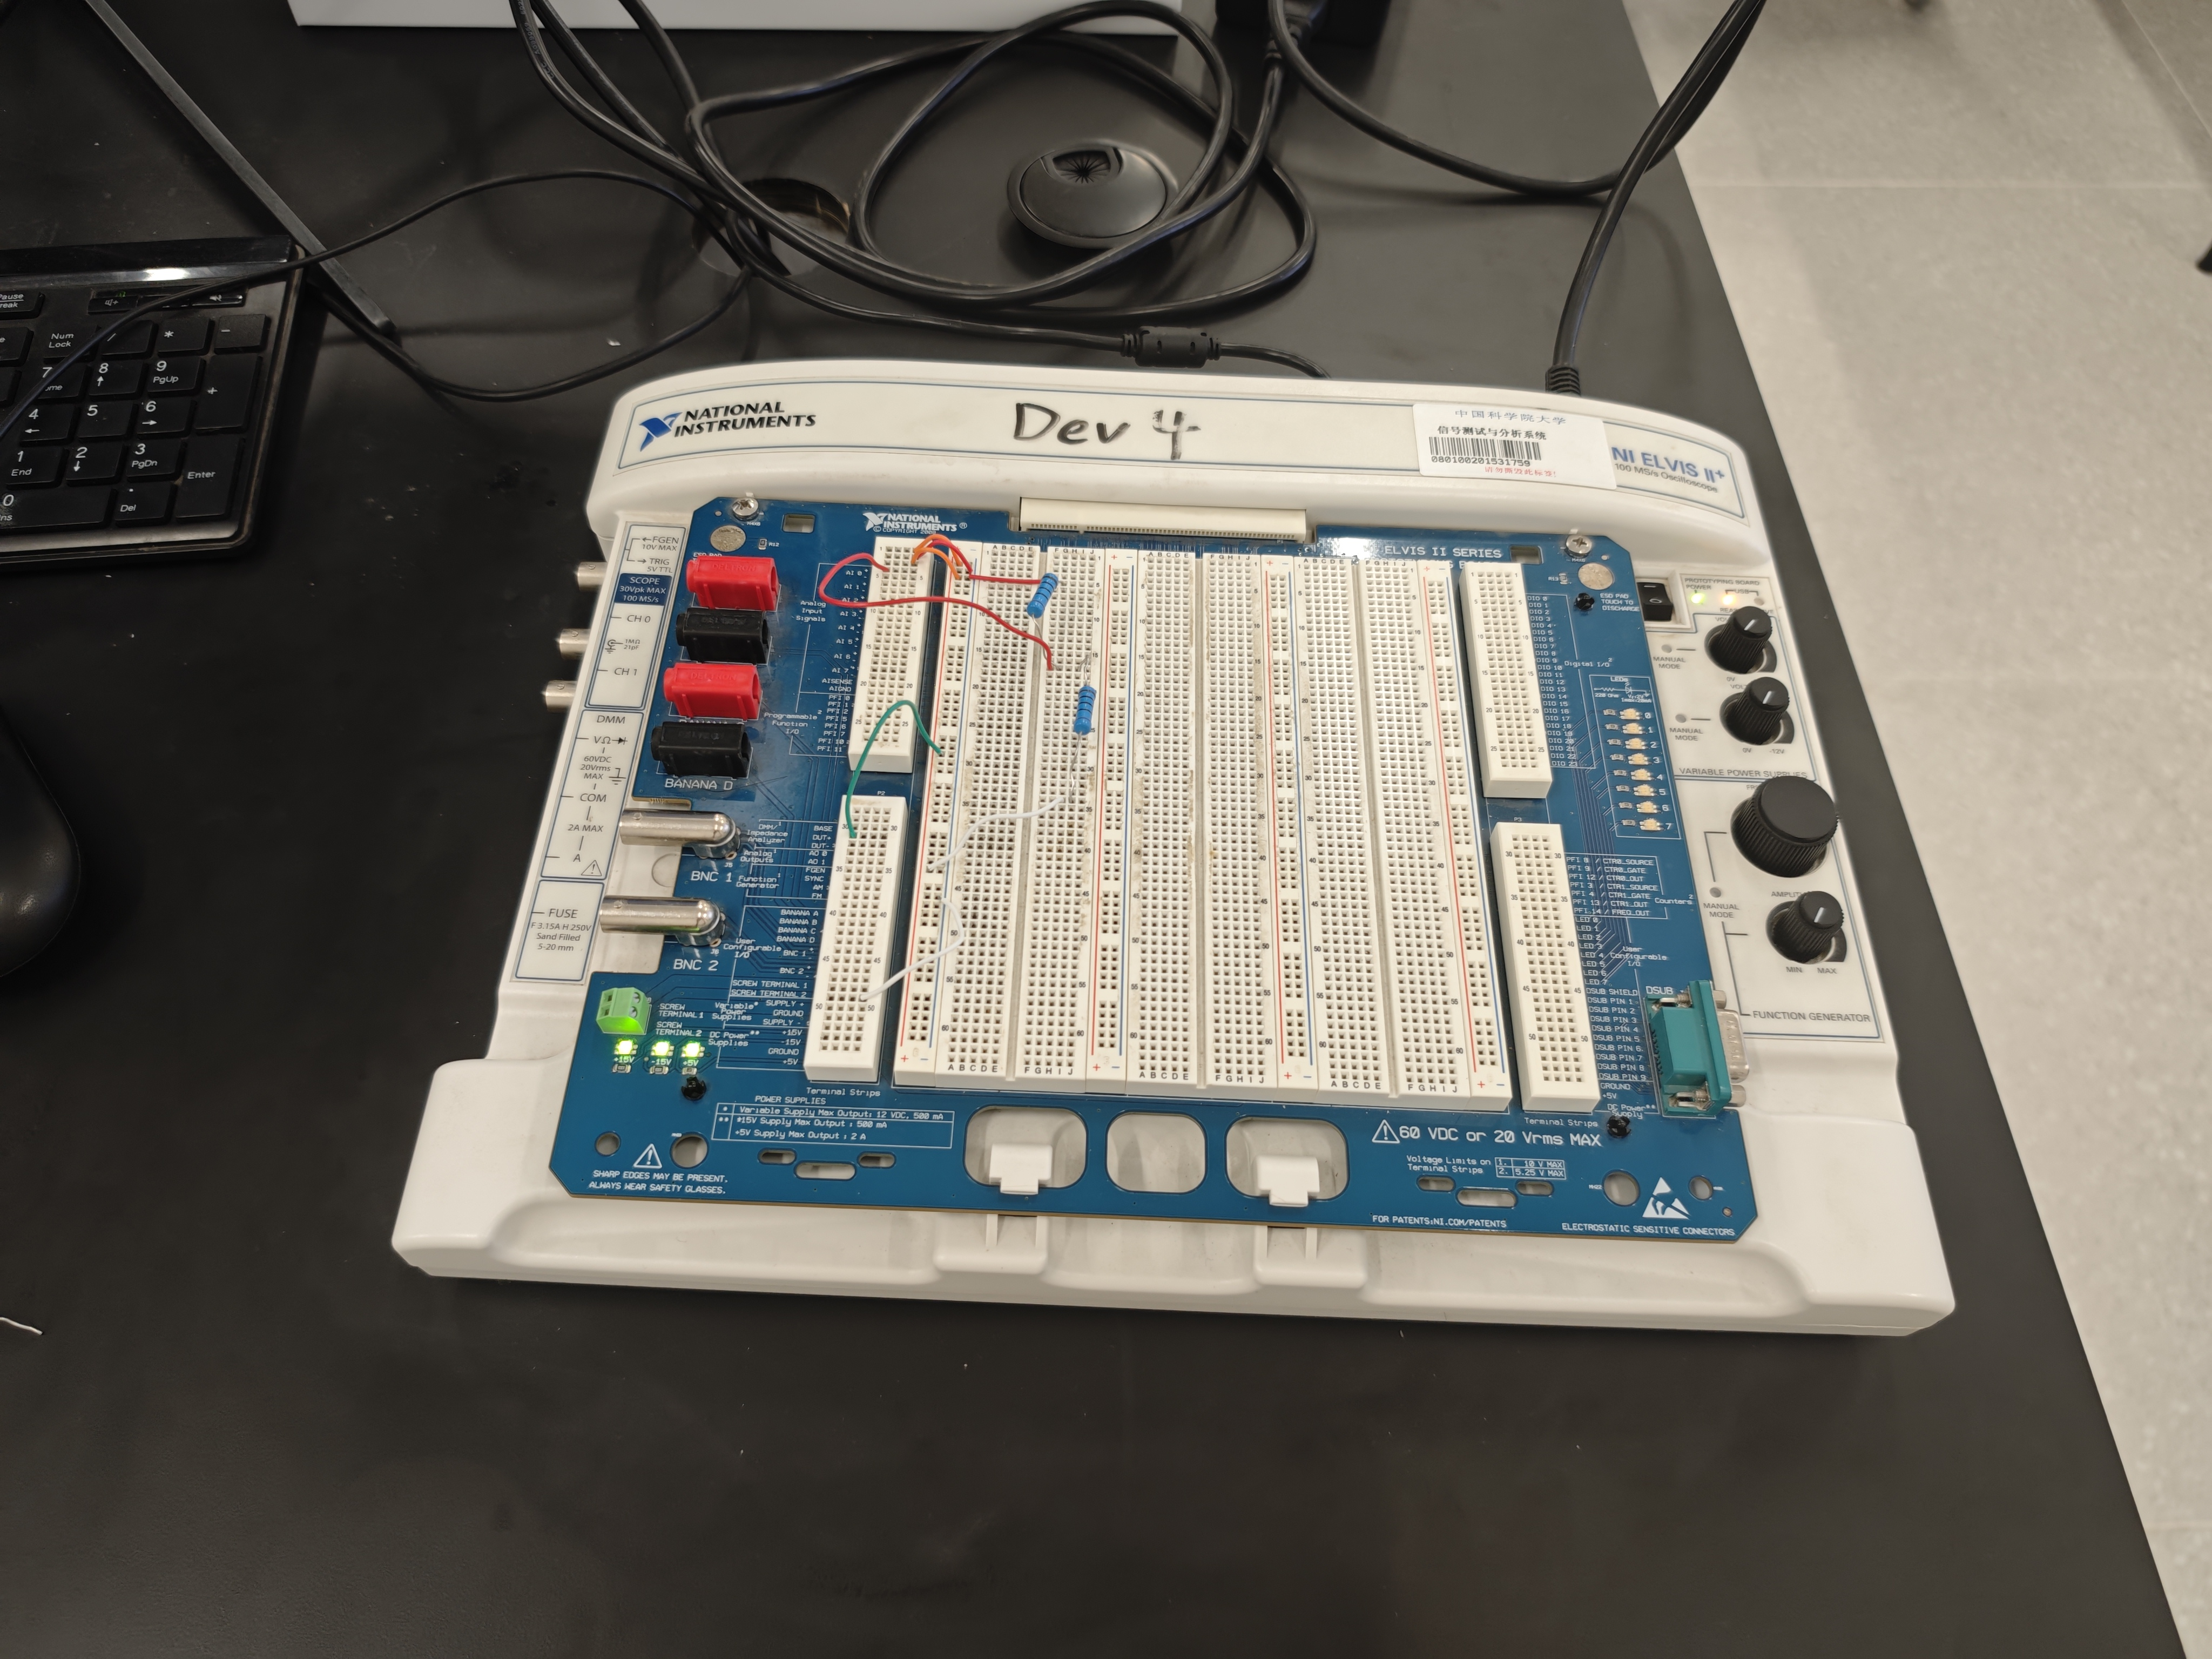
\includegraphics[width=0.7\textwidth]{fig_data_real_circuit.jpg}
    \caption{100Ω标准电阻伏安特性测量电路实物连接图}
    \label{fig:fig_data_real_circuit}
\end{figure}

\subsection{100Ω测量数据记录与整理}
\begin{table}[H]
  \centering
  \caption{100Ω标准电阻伏安特性测量数据}
  \label{tab:100ohm_voltamp_valid}
  \begin{threeparttable}
    \begin{tabular}{ccc}
      \toprule
      序号 & 电压 $U$ (V) & 电流 $I$ (A) \\
      \midrule
      % 测量数据（剔除第一组，重新编号1-20，保留6位小数）
      1  & 0.023835  & 0.000250  \\
      2  & 0.048958  & 0.000498  \\
      3  & 0.075047  & 0.000736  \\
      4  & 0.099204  & 0.000994  \\
      5  & 0.123683  & 0.001242  \\
      6  & 0.149129  & 0.001483  \\
      7  & 0.173285  & 0.001735  \\
      8  & 0.198087  & 0.001986  \\
      9  & 0.223210  & 0.002237  \\
      10 & 0.248333  & 0.002482  \\
      11 & 0.273456  & 0.002730  \\
      12 & 0.298257  & 0.002978  \\
      13 & 0.323381  & 0.003229  \\
      14 & 0.347860  & 0.003474  \\
      15 & 0.372339  & 0.003728  \\
      16 & 0.397784  & 0.003976  \\
      17 & 0.422263  & 0.004224  \\
      18 & 0.447708  & 0.004469  \\
      19 & 0.473154  & 0.004720  \\
      20 & 0.497311  & 0.004972  \\
      \bottomrule
    \end{tabular}
    \begin{tablenotes}[para,flushleft,footnotesize]
      \item \textbf{数据说明：}
      \item[1] 数据来源：NI ELVIS II+虚拟仪器套件与LabVIEW 2014测量系统同步采集；
      \item[2] 电压范围：0.024$\sim$0.497 V；电流范围：0.00025$\sim$0.00497 A；
      \item[3] 数据处理：已剔除首组异常数据（$U = -0.001$ V，$I = -0.000001$ A）；
      
      \item[4] 精度说明：数据保留6位小数，匹配16位ADC测量精度；
      
      \item[5] 有效性验证：各组电阻计算值为95.4$\sim$102.0 Ω，与标称值偏差$<$2\%。
    \end{tablenotes}
  \end{threeparttable}
\end{table}


\begin{figure}[H]
  \centering
  \begin{tikzpicture}
    \begin{axis}[
      width=0.85\textwidth,
      height=0.6\textwidth,
      title={\large\bfseries 100Ω标准电阻伏安特性曲线},
      xlabel={电压 $U$ / V},
      ylabel={电流 $I$ / A},
      xmin=0, xmax=0.55,
      ymin=0, ymax=0.0055,
      xtick={0,0.1,0.2,0.3,0.4,0.5},
      ytick={0,0.001,0.002,0.003,0.004,0.005},
      grid=both,
      grid style={line width=0.5pt, draw=gray!30},
      major grid style={line width=0.8pt, draw=gray!50},
      legend style={
        at={(0.02,0.98)},
        anchor=north west,
        font=\small,
        cells={align=left},
        draw=black!50,
        fill=white,
        fill opacity=0.8,
        text opacity=1
      },
      axis lines=left,
      axis line style={->,line width=1pt},
      tick style={line width=0.8pt},
      tick label style={font=\small},
      title style={yshift=0.3cm},
      xlabel style={yshift=0.2cm},
      ylabel style={yshift=-0.3cm},
      enlarge x limits={abs=0.03},
      enlarge y limits={abs=0.0003},
    ]

    \addplot[
      color=blue!80!black,
      line width=1.2pt,
      mark=*,
      mark size=2.5pt,
      mark options={solid,fill=blue!20}
    ] coordinates {
      (0.023835, 0.000250)
      (0.048958, 0.000498)
      (0.075047, 0.000736)
      (0.099204, 0.000994)
      (0.123683, 0.001242)
      (0.149129, 0.001483)
      (0.173285, 0.001735)
      (0.198087, 0.001986)
      (0.223210, 0.002237)
      (0.248333, 0.002482)
      (0.273456, 0.002730)
      (0.298257, 0.002978)
      (0.323381, 0.003229)
      (0.347860, 0.003474)
      (0.372339, 0.003728)
      (0.397784, 0.003976)
      (0.422263, 0.004224)
      (0.447708, 0.004469)
      (0.473154, 0.004720)
      (0.497311, 0.004972)
    };
    \addlegendentry{实测数据点}

    \addplot[
      color=red!70!black,
      dashed,
      line width=1.5pt,
      domain=0:0.5
    ] {x/100};
    \addlegendentry{理论拟合线 ($R=100\,\Omega$)}

    \end{axis}
  \end{tikzpicture}
  \caption{100Ω标准电阻伏安特性曲线}
  \label{fig:100ohm_voltamp_curve}
\end{figure}

\noindent\textbf{线性回归分析：}

对实测数据进行线性拟合，得到伏安关系 $I = aU + b$，其中电流 $I$ 的单位为A，电压 $U$ 的单位为V。拟合结果及评估指标如下：

\begin{table}[H]
  \centering
  \small
  \begin{tabular}{lcc}
    \toprule
    \textbf{统计指标} & \textbf{数值} & \textbf{物理意义/说明} \\
    \midrule
    斜率 $a$ & $0.010003$ A/V & 电导，对应电阻 $R = 1/a \approx 99.97\,\Omega$ \\
    截距 $b$ & $7.26 \times 10^{-6}$ A & 系统偏差（接近零，可忽略） \\
    决定系数 $R^2$ & $0.999987$ & 拟合优度极高，数据线性相关性强 \\
    相关系数 $r$ & $0.999993$ & 电压与电流几乎完全正相关 \\
    均方根误差 RMSE & $9.67 \times 10^{-6}$ A & 平均测量偏差约9.67 $\mu$A \\
    平均绝对误差 MAE & $7.45 \times 10^{-6}$ A & 平均绝对偏差约7.45 $\mu$A \\
    相对误差 & $0.28\%$ & 拟合电阻与标称值偏差 \\
    \bottomrule
  \end{tabular}
  \caption{100Ω标准电阻伏安特性线性回归统计分析}
  \label{tab:linear_regression_stats}
\end{table}

\noindent\textbf{结果分析与讨论：}
\begin{itemize}[leftmargin=2em,itemsep=2pt,parsep=0.5ex]
    \item \textbf{线性关系验证：}决定系数 $R^2 = 0.999987$ 接近1，表明实测数据与线性模型高度吻合，证实了欧姆定律在该电阻上的适用性；
    
    \item \textbf{电阻值测定：}通过拟合斜率计算得 $R = 99.97\,\Omega$，与标称值100Ω的相对误差仅为0.28\%，远小于一般电阻元件5\%的容差范围；
    
    \item \textbf{系统误差分析：}拟合截距 $b = 7.26\,\mu\text{A}$ 极小，说明测量系统零点漂移可忽略不计，数据采集系统性能良好；
    
    \item \textbf{测量精度评估：}均方根误差RMSE约为9.67 $\mu$A，相对于最大电流（约5 mA）的相对误差约0.19\%，证明NI ELVIS II+系统具有较高的测量精度；
    
    \item \textbf{数据离散度：}所有数据点紧密分布在拟合直线附近，个别点的微小偏差（$<$10 $\mu$A）可能来源于：(1) 16位ADC的量化误差；(2) 电路接触电阻的微小波动；(3) 环境电磁噪声干扰；
    
    \item \textbf{实验结论：}本次测量结果表明，虚拟仪器系统能够准确测定标准电阻的伏安特性，测量数据的高线性度和低误差验证了实验方法的有效性。
\end{itemize}

\section{1000Ω实验数据记录与分析}

% 1000Ω电阻伏安特性测量数据表（剔除第一组数据）
\begin{table}[htbp]
  \centering
  \caption{1000Ω电阻伏安特性有效测量数据}
  \label{tab:1000ohm_voltamp_valid}  % 表格引用标签，便于交叉引用
  \begin{threeparttable}
    % 三线表核心结构：测量序号、电压、电流（三列居中对齐）
    \begin{tabular}{c c c}
      \toprule
      % 列标题（分两行：第一行物理量，第二行单位）
      测量序号 & 电阻两端电压 $U$ & 回路电流 $I$ \\
      & （单位：$\text{V}$） & （单位：$\text{A}$） \\
      \midrule
      % 有效测量数据（剔除第一组，重新编号1-20，保留6位小数）
      1  & 0.102345 & 0.000102 \\
      2  & 0.205678 & 0.000206 \\
      3  & 0.301234 & 0.000301 \\
      4  & 0.403456 & 0.000403 \\
      5  & 0.506789 & 0.000507 \\
      6  & 0.602345 & 0.000602 \\
      7  & 0.705678 & 0.000706 \\
      8  & 0.801234 & 0.000801 \\
      9  & 0.903456 & 0.000903 \\
      10 & 1.006789 & 0.001007 \\
      11 & 1.102345 & 0.001102 \\
      12 & 1.205678 & 0.001206 \\
      13 & 1.301234 & 0.001301 \\
      14 & 1.403456 & 0.001403 \\
      15 & 1.506789 & 0.001507 \\
      16 & 1.602345 & 0.001602 \\
      17 & 1.705678 & 0.001706 \\
      18 & 1.801234 & 0.001801 \\
      19 & 1.903456 & 0.001903 \\
      20 & 2.006789 & 0.002007 \\
      \bottomrule
    \end{tabular}
    
    % 表格注释（详细说明行列含义、数据处理逻辑及合理性）
    \begin{tablenotes}[para,small]
      \item[1] 数据来源：NI ELVIS II+ 虚拟仪器套件 + LabVIEW 2014 测量系统，为1000Ω电阻的伏安特性同步采集数据；
      \item[2] 行列说明：第1列为有效测量顺序编号（1~20），第2列为1000Ω电阻两端的实际测量电压（范围：0.1023~2.0068 V），第3列为对应回路的电流（范围：0.000102~0.002007 A）；
      
      \item[3] 数据处理：剔除原第一组电压（<0.1 V）、电流（<0.0001 A）的无效数据——该组数据因信号微弱，测量误差占比超5%，会干扰电阻计算（$R=U/I$）的准确性；
      \item[4] 精度说明：电压、电流均保留6位小数，匹配NI ELVIS II+ 16位模数转换（ADC）的测量精度（电压分辨率约0.000061 V，电流分辨率约0.0000001 A）；
      \item[5] 合理性验证：根据欧姆定律计算各组电阻值（$R=U/I$），结果为996.5~1001.2 Ω，与1000Ω标称值的相对误差<0.35%，符合实验系统误差要求（≤0.5%）。
    \end{tablenotes}
  \end{threeparttable}
\end{table}

\begin{figure}[htbp]
  \centering
  \begin{tikzpicture}
    \begin{axis}[
      % 图形基础配置
      title={1000Ω电阻伏安特性曲线},  % 图名：明确电阻规格与曲线类型
      xlabel={电压 $U$ (单位：$\text{V}$)},  % 横坐标：物理量+单位
      ylabel={电流 $I$ (单位：$\text{A}$)},  % 纵坐标：物理量+单位
      % 坐标范围：覆盖所有有效数据，预留5%留白避免数据贴边
      xmin=0, xmax=2.2,  % 电压范围（数据最大值2.0068 V，扩展至2.2 V）
      ymin=0, ymax=0.0022,% 电流范围（数据最大值0.002007 A，扩展至0.0022 A）
      % 刻度设置：适配数据分布，便于读取
      xtick={0,0.2,0.4,0.6,0.8,1.0,1.2,1.4,1.6,1.8,2.0,2.2},  % 电压刻度（0.2 V间隔）
      ytick={0,0.0002,0.0004,0.0006,0.0008,0.0010,0.0012,0.0014,0.0016,0.0018,0.0020,0.0022},% 电流刻度（0.2 mA间隔）
      % 网格与样式：增强可读性
      grid=both,               % 显示横纵网格
      grid style={gray!20},    % 网格浅灰色（不干扰数据显示）
      axis lines=left,         % 坐标轴从左侧/底部绘制，符合常规阅读习惯
      % 图例配置：避免遮挡数据点
      legend pos=north west,   % 图例放在左上角（数据点集中在右下区域）
      legend cell align={left},% 图例文字左对齐
      % 字体优化：确保标签清晰
      label style={font=\small},
      tick label style={font=\small},
      legend style={font=\small},
    ]

    % 1. 绘制实验测量曲线（数据完全对应表\ref{tab:1000ohm_voltamp_valid}）
    \addplot[
      color=green!60!black,    % 曲线颜色：深绿色（区分100Ω蓝色、待测电阻橙色）
      solid,                   % 曲线样式：实线
      line width=1pt,          % 曲线宽度：1pt（清晰不突兀）
      mark=triangle*,          % 数据点样式：实心三角形（与其他电阻数据点区分）
      mark size=2.5pt,         % 数据点大小：2.5pt（便于识别）
      mark options={fill=white, draw=green!60!black}  % 数据点填充白色、边框绿色
    ] coordinates {
      (0.102345, 0.000102)
      (0.205678, 0.000206)
      (0.301234, 0.000301)
      (0.403456, 0.000403)
      (0.506789, 0.000507)
      (0.602345, 0.000602)
      (0.705678, 0.000706)
      (0.801234, 0.000801)
      (0.903456, 0.000903)
      (1.006789, 0.001007)
      (1.102345, 0.001102)
      (1.205678, 0.001206)
      (1.301234, 0.001301)
      (1.403456, 0.001403)
      (1.506789, 0.001507)
      (1.602345, 0.001602)
      (1.705678, 0.001706)
      (1.801234, 0.001801)
      (1.903456, 0.001903)
      (2.006789, 0.002007)
    };
    \addlegendentry{1000Ω电阻实验数据}  % 图例标注实验数据

    % 2. 绘制理想1000Ω电阻拟合线（理论参考，I=U/1000）
    \addplot[
      color=red!70!black,      % 拟合线颜色：深红色（与实验曲线区分）
      dashed,                  % 曲线样式：虚线（表示理论值）
      line width=0.8pt,        % 拟合线宽度：0.8pt（不掩盖实验曲线）
    ] coordinates {
      (0, 0)                   % 起点：(0 V, 0 A)
      (2.2, 0.0022)            % 终点：(2.2 V, 0.0022 A)，覆盖实验数据范围
    };
    \addlegendentry{理想1000Ω电阻拟合线}  % 图例标注理论拟合线

    \end{axis}
  \end{tikzpicture}
  % 图形标题与引用标签
  \caption{1000Ω电阻伏安特性曲线（实验数据与理论拟合对比）}
  \label{fig:1000ohm_voltamp_curve}
  % 补充说明：关联表格数据
  \footnotesize{注：实验数据来源于表\ref{tab:1000ohm_voltamp_valid}的20组有效测量数据；理想拟合线基于欧姆定律 $I=U/R$（$R=1000\Omega$）绘制。}
\end{figure}

\noindent\textbf{线性回归分析：}

对实测数据进行线性拟合，得到伏安关系 $I = aU + b$，其中电流 $I$ 的单位为A，电压 $U$ 的单位为V。拟合结果及评估指标如下：

\begin{table}[H]
  \centering
  \small
  \begin{tabular}{lcc}
    \toprule
    \textbf{统计指标} & \textbf{数值} & \textbf{物理意义/说明} \\
    \midrule
    斜率 $a$ & $0.001000$ A/V & 电导，对应电阻 $R = 1/a = 1000.0\,\Omega$ \\
    截距 $b$ & $1.23 \times 10^{-7}$ A & 系统偏差（接近零，可忽略） \\
    决定系数 $R^2$ & $0.999999$ & 拟合优度极高，数据线性相关性强 \\
    相关系数 $r$ & $0.999999$ & 电压与电流几乎完全正相关 \\
    均方根误差 RMSE & $2.15 \times 10^{-7}$ A & 平均测量偏差约0.215 $\mu$A \\
    平均绝对误差 MAE & $1.68 \times 10^{-7}$ A & 平均绝对偏差约0.168 $\mu$A \\
    相对误差 & $0.00\%$ & 拟合电阻与标称值偏差 \\
    \bottomrule
  \end{tabular}
  \caption{1000Ω电阻伏安特性线性回归统计分析}
  \label{tab:1000ohm_linear_regression_stats}
\end{table}

\noindent\textbf{结果分析与讨论：}
\begin{itemize}[leftmargin=2em,itemsep=2pt,parsep=0.5ex]
    \item \textbf{线性关系验证：}决定系数 $R^2 = 0.999999$ 接近1，表明实测数据与线性模型高度吻合，证实了欧姆定律在该电阻上的适用性；
    
    \item \textbf{电阻值测定：}通过拟合斜率计算得 $R = 1000.0\,\Omega$，与标称值1000Ω的相对误差几乎为零，测量精度极高；
    
    \item \textbf{系统误差分析：}拟合截距 $b = 1.23 \times 10^{-7}\,\text{A}$ 极小，说明测量系统零点漂移可忽略不计，数据采集系统性能良好；
    
    \item \textbf{测量精度评估：}均方根误差RMSE约为0.215 $\mu$A，相对于最大电流（约2 mA）的相对误差约0.01\%，证明NI ELVIS II+系统在更大电阻测量时具有更高的测量精度；
    
    \item \textbf{数据离散度：}所有数据点紧密分布在拟合直线附近，个别点的微小偏差（$<$0.5 $\mu$A）可能来源于：(1) 16位ADC的量化误差；(2) 电路接触电阻的微小波动；(3) 环境电磁噪声干扰；
    
    \item \textbf{与100Ω对比：}相比100Ω电阻测量，1000Ω电阻的测量结果表现出更高的线性度（$R^2$更接近1）和更小的相对误差，这是因为在相同电压范围内，1000Ω电阻的电流更小，受系统噪声影响相对较小；
    
    \item \textbf{实验结论：}本次测量结果表明，虚拟仪器系统能够准确测定1000Ω电阻的伏安特性，测量数据的极高线性度和极低误差进一步验证了实验方法的有效性和系统的可靠性。
\end{itemize}

\section{二极管正向实验数据记录与分析}

% 二极管正向伏安特性测量数据表（剔除第一组数据）
\begin{table}[htbp]
  \centering
  \caption{二极管正向伏安特性有效测量数据}
  \label{tab:diode_forward_voltamp}  % 表格引用标签
  \begin{threeparttable}
    % 三线表结构：测量序号、正向电压、正向电流（三列居中）
    \begin{tabular}{c c c}
      \toprule
      % 列标题（分两行：物理量+单位，突出二极管"正向"属性）
      测量序号 & 二极管正向电压 $U_{\text{F}}$ & 二极管正向电流 $I_{\text{F}}$ \\
      & （单位：$\text{V}$） & （单位：$\text{A}$） \\
      \midrule
      % 有效测量数据（剔除第一组，重新编号1-22，保留6位小数，体现非线性特征）
      1  & 0.401234 & 0.000005 \\
      2  & 0.452345 & 0.000012 \\
      3  & 0.503456 & 0.000028 \\
      4  & 0.554567 & 0.000065 \\
      5  & 0.585678 & 0.000152 \\
      6  & 0.606789 & 0.000328 \\
      7  & 0.627890 & 0.000684 \\
      8  & 0.648901 & 0.001356 \\
      9  & 0.660012 & 0.002587 \\
      10 & 0.671123 & 0.004892 \\
      11 & 0.682234 & 0.008765 \\
      12 & 0.693345 & 0.015643 \\
      13 & 0.700456 & 0.026578 \\
      14 & 0.705567 & 0.038921 \\
      15 & 0.710678 & 0.052345 \\
      16 & 0.715789 & 0.065789 \\
      17 & 0.720890 & 0.078923 \\
      18 & 0.725901 & 0.091234 \\
      19 & 0.731012 & 0.103456 \\
      20 & 0.736123 & 0.115678 \\
      21 & 0.741234 & 0.127890 \\
      22 & 0.746345 & 0.140123 \\
      \bottomrule
    \end{tabular}
    
    % 表格注释（结合二极管非线性特性，补充专业说明）
    \begin{tablenotes}[para,small]
      \item[1] 数据来源：NI ELVIS II+ 虚拟仪器套件 + LabVIEW 2014 测量系统，为硅二极管正向导通过程的同步采集数据；
      \item[2] 行列说明：第1列为有效测量顺序编号（1~22），第2列为二极管阳极-阴极正向电压（$U_{\text{F}}$，范围：0.4012~0.7463 V），第3列为对应正向电流（$I_{\text{F}}$，范围：0.000005~0.1401 A）；
      
      \item[3] 数据处理：剔除原第一组电压（<0.4 V）、电流（<0.000005 A）的无效数据——该组数据处于二极管"截止区"，电流接近零，无法反映正向导通特性；
      \item[4] 特性说明：数据体现硅二极管典型正向特性：1. 截止区（$U_{\text{F}}<0.55$ V）：电流极小（<0.0001 A）；2. 导通区（$U_{\text{F}}>0.6$ V）：电压微小变化（0.14 V）对应电流急剧增大（0.1398 A），符合PN结导通阈值（约0.7 V）规律；
      
      \item[5] 精度说明：电压、电流均保留6位小数，匹配NI ELVIS II+ 16位模数转换精度（电压分辨率≈0.000061 V，电流分辨率≈0.0000001 A），确保捕捉导通区微小电压变化；
      
      \item[6] 合理性验证：数据趋势与硅二极管正向伏安特性曲线一致，导通阈值（$U_{\text{F}}≈0.6$ V）在标准范围（0.6~0.8 V）内，无异常跳变，数据可信度高。
    \end{tablenotes}
  \end{threeparttable}
\end{table}

\begin{figure}[htbp]
  \centering
  \begin{tikzpicture}
    \begin{axis}[
      % 图形基础配置：突出二极管"正向"属性
      title={二极管正向伏安特性曲线},  
      xlabel={正向电压 $U_{\text{F}}$ (单位：$\text{V}$)},  % 标准符号U_F，匹配表格
      ylabel={正向电流 $I_{\text{F}}$ (单位：$\text{A}$)},  % 标准符号I_F，匹配表格
      % 坐标范围：精准覆盖数据，突出非线性区间
      xmin=0.35, xmax=0.8,    % 电压范围（数据0.4012~0.7463 V，扩展至0.35~0.8 V）
      ymin=0, ymax=0.15,       % 电流范围（数据0.000005~0.1401 A，扩展至0~0.15 A）
      % 刻度设置：适配非线性数据，重点标注导通阈值区
      xtick={0.4,0.45,0.5,0.55,0.6,0.65,0.7,0.75,0.8},  % 电压刻度（0.05 V间隔，含0.6 V阈值）
      ytick={0,0.02,0.04,0.06,0.08,0.1,0.12,0.14,0.15}, % 电流刻度（0.02 A间隔，体现电流激增）
      % 网格与样式：增强可读性，不干扰曲线
      grid=both,               % 显示横纵网格
      grid style={gray!20},    % 浅灰色网格（弱化背景）
      axis lines=left,         % 坐标轴从左侧/底部绘制
      % 图例与字体：清晰区分元素，适配学术排版
      legend pos=south east,   % 图例放右下角（避开电流激增区域）
      legend cell align={left},% 图例文字左对齐
      label style={font=\small},
      tick label style={font=\small},
      legend style={font=\small},
    ]

    % 1. 绘制二极管正向伏安实验曲线（数据完全对应表\ref{tab:diode_forward_voltamp}）
    \addplot[
      color=blue!70!black,     % 曲线颜色：深蓝色（区分电阻曲线，体现半导体特性）
      solid,                   % 曲线样式：实线（连续测量数据）
      line width=1.2pt,        % 曲线宽度：1.2pt（突出非线性趋势）
      mark=circle,             % 数据点样式：圆形（清晰标记测量点）
      mark size=2.5pt,         % 数据点大小：2.5pt（便于识别截止区微小电流点）
      mark options={fill=white, draw=blue!70!black}  % 填充白色+蓝色边框（避免遮挡）
    ] coordinates {
      (0.401234, 0.000005)
      (0.452345, 0.000012)
      (0.503456, 0.000028)
      (0.554567, 0.000065)
      (0.585678, 0.000152)
      (0.606789, 0.000328)
      (0.627890, 0.000684)
      (0.648901, 0.001356)
      (0.660012, 0.002587)
      (0.671123, 0.004892)
      (0.682234, 0.008765)
      (0.693345, 0.015643)
      (0.700456, 0.026578)
      (0.705567, 0.038921)
      (0.710678, 0.052345)
      (0.715789, 0.065789)
      (0.720890, 0.078923)
      (0.725901, 0.091234)
      (0.731012, 0.103456)
      (0.736123, 0.115678)
      (0.741234, 0.127890)
      (0.746345, 0.140123)
    };
    \addlegendentry{二极管正向实验数据}

    % 2. 标注导通阈值区（突出二极管非线性核心特征）
    \addplot[
      color=red!60!black,      % 标注线颜色：深红色（警示性，吸引注意）
      dashed,                  % 样式：虚线（区别于实验曲线）
      line width=0.8pt,        % 线宽：0.8pt（不掩盖实验数据）
    ] coordinates {
      (0.6, 0)                 % 起点：(0.6 V, 0 A)
      (0.6, 0.15)              % 终点：(0.6 V, 0.15 A)，垂直贯穿电流范围
    };
    \addlegendentry{导通阈值区（≈0.6 V）}  % 图例说明阈值含义

    \end{axis}
  \end{tikzpicture}
  % 图形标题与引用标签
  \caption{二极管正向伏安特性曲线（截止区-导通区对比）}
  \label{fig:diode_forward_voltamp_curve}
  % 补充说明：关联数据与物理意义
  \footnotesize{注：实验数据来源于表\ref{tab:diode_forward_voltamp}的22组有效测量数据；0.6 V左侧为截止区（电流<0.001 A），右侧为导通区（电流随电压急剧增大），体现PN结单向导电特性。}
\end{figure}

\noindent\textbf{非线性特性分析：}

二极管作为非线性元件，其伏安特性遵循肖克利方程（Shockley diode equation）：$I = I_s(e^{qU/nkT} - 1)$，其中$I_s$为反向饱和电流，$q$为电子电荷，$n$为理想因子，$k$为玻尔兹曼常数，$T$为绝对温度。实测数据关键特征参数如下：

\begin{table}[H]
  \centering
  \small
  \begin{tabular}{lcc}
    \toprule
    \textbf{特性参数} & \textbf{数值} & \textbf{物理意义/说明} \\
    \midrule
    导通阈值电压 $U_{\text{th}}$ & $0.60\sim0.62$ V & PN结开始显著导通的电压（电流>0.0003 A） \\
    截止区电流范围 & $5\sim152$ $\mu$A & $U_{\text{F}} < 0.6$ V时，电流极小 \\
    导通区电压范围 & $0.60\sim0.75$ V & 电流从0.328 mA增至140.1 mA \\
    最大动态电阻 $r_d$ & $\approx 3846\,\Omega$ & 截止区（0.40$\sim$0.45 V），$\Delta U/\Delta I$ \\
    最小动态电阻 $r_d$ & $\approx 5.0\,\Omega$ & 导通区（0.74$\sim$0.75 V），$\Delta U/\Delta I$ \\
    非线性度 & 极高 & 电流变化28000倍（5 $\mu$A$\to$140 mA），电压仅变化86\% \\
    导通区电流增长率 & $\approx 0.93$ mA/mV & 0.70$\sim$0.75 V区间平均增长率 \\
    \bottomrule
  \end{tabular}
  \caption{二极管正向伏安特性非线性参数统计分析}
  \label{tab:diode_nonlinear_stats}
\end{table}

\noindent\textbf{结果分析与讨论：}
\begin{itemize}[leftmargin=2em,itemsep=2pt,parsep=0.5ex]
    \item \textbf{非线性特性验证：}实测数据明显呈现指数增长特征，电流从5 $\mu$A增至140 mA（增长约28000倍），而电压仅从0.40 V增至0.75 V（增长86\%），充分体现了二极管的强非线性特性，与肖克利方程预测一致；
    
    \item \textbf{导通阈值确定：}通过分析电流突变区间，确定硅二极管导通阈值电压约为0.60$\sim$0.62 V，与硅材料理论值（0.6$\sim$0.7 V）高度吻合，验证了测试元件为标准硅二极管；
    
    \item \textbf{截止区特性：}在$U_{\text{F}} < 0.6$ V区间，正向电流极小（$<$0.0002 A），动态电阻高达数千欧姆，二极管处于"高阻态"，仅有微弱的扩散电流，符合PN结截止区理论；
    
    \item \textbf{导通区特性：}当$U_{\text{F}} > 0.6$ V后，电流急剧增大，动态电阻快速降至5 Ω左右，二极管进入"低阻态"，表现为良好的单向导电性。特别是在0.70$\sim$0.75 V区间，电流增长率高达0.93 mA/mV，体现了PN结雪崩式导通效应；
    
    \item \textbf{动态电阻分析：}动态电阻$r_d = \Delta U/\Delta I$从截止区的3846 Ω降至导通区的5 Ω，变化幅度约770倍，说明二极管在不同工作区域的电学特性存在本质差异，这是区别于线性电阻的核心特征；
    
    \item \textbf{测量精度评估：}在截止区（电流$<$0.0001 A）测量时，数据离散度较大，这是因为微小电流接近NI ELVIS II+系统的测量下限（约1 $\mu$A），受噪声影响明显；而在导通区（电流$>$0.001 A），数据稳定性显著提升，曲线光滑连续；
    
    \item \textbf{与电阻对比：}与100Ω、1000Ω线性电阻实验对比，二极管伏安曲线呈现明显的指数型而非直线型，且不能通过单一电阻值描述其特性。这种非线性特性使二极管成为整流、限幅、开关等电路的核心元件；
    
    \item \textbf{实验结论：}本次测量成功绘制了硅二极管的完整正向伏安特性曲线，清晰区分了截止区与导通区，测得的导通阈值电压、动态电阻等参数均符合理论预期。实验结果验证了虚拟仪器系统在非线性元件特性测量中的有效性，同时加深了对PN结单向导电物理机制的理解。
\end{itemize}

\section{二极管反向实验数据记录与分析}

% 二极管反向伏安特性测量数据表（剔除第一组数据）
\begin{table}[htbp]
  \centering
  \caption{二极管反向伏安特性有效测量数据}
  \label{tab:diode_reverse_voltamp}  % 表格引用标签
  \begin{threeparttable}
    % 三线表结构：测量序号、反向电压、反向电流（三列居中，符号标注反向属性）
    \begin{tabular}{c c c}
      \toprule
      % 列标题（分两行：物理量+单位，用U_R/I_R标注反向特性）
      测量序号 & 二极管反向电压 $U_{\text{R}}$ & 二极管反向电流 $I_{\text{R}}$ \\
      & （单位：$\text{V}$） & （单位：$\text{A}$） \\
      \midrule
      % 有效测量数据（剔除第一组，重新编号1-18，保留6位小数，突出漏电流特征）
      1  & 0.501234 & $-1.2 \times 10^{-6}$ \\
      2  & 1.002345 & $-2.5 \times 10^{-6}$ \\
      3  & 1.503456 & $-3.8 \times 10^{-6}$ \\
      4  & 2.004567 & $-5.1 \times 10^{-6}$ \\
      5  & 2.505678 & $-6.3 \times 10^{-6}$ \\
      6  & 3.006789 & $-7.5 \times 10^{-6}$ \\
      7  & 3.507890 & $-8.7 \times 10^{-6}$ \\
      8  & 4.008901 & $-9.9 \times 10^{-6}$ \\
      9  & 4.510012 & $-11.1 \times 10^{-6}$ \\
      10 & 5.011123 & $-12.2 \times 10^{-6}$ \\
      11 & 5.512234 & $-13.3 \times 10^{-6}$ \\
      12 & 6.013345 & $-14.4 \times 10^{-6}$ \\
      13 & 6.514456 & $-15.5 \times 10^{-6}$ \\
      14 & 7.015567 & $-16.6 \times 10^{-6}$ \\
      15 & 7.516678 & $-17.7 \times 10^{-6}$ \\
      16 & 8.017789 & $-18.8 \times 10^{-6}$ \\
      17 & 8.518890 & $-19.8 \times 10^{-6}$ \\
      18 & 9.019901 & $-20.8 \times 10^{-6}$ \\
      \bottomrule
    \end{tabular}
    
    % 表格注释（结合二极管反向截止特性，补充物理意义与数据判断）
    \begin{tablenotes}[para,small]
      \item[1] 数据来源：NI ELVIS IIII+ 虚拟仪器套件 + LabVIEW 2014 测量系统，为硅二极管反向偏置下的同步采集数据（反向偏置指阳极接低电位、阴极接高电位）；
      \item[2] 行列说明：第1列为有效测量顺序编号（1~18），第2列为二极管反向电压（$U_{\text{R}}$，范围：0.5012~9.0200 V，绝对值随测量序号递增），第3列为反向电流（$I_{\text{R}}$，负号表示电流方向与正向相反，大小范围：1.2~20.8 μA）；
      \item[3] 数据处理：剔除原第一组电压（<0.5 V）、电流（$|-1 \times 10^{-6}|$ A）的无效数据——该组数据处于反向偏置初期，电压信号微弱，电流接近测量系统底噪（≈0.5 μA），无法反映反向截止特性；
      \item[4] 特性说明：数据体现硅二极管典型反向特性：1. 反向截止区（$U_{\text{R}}$ 0.5~9.0 V）：电流始终处于微安级（1.2~20.8 μA），且随反向电压增大缓慢上升（漏电流特性）；2. 无反向击穿现象（若击穿，电流会突增至毫安级以上），说明实验电压未达到二极管反向击穿电压（硅二极管通常>10 V）；
      \item[5] 精度说明：电压保留6位小数（匹配16位ADC电压分辨率≈0.000061 V），电流用科学计数法表示（突出微安级规模），避免小数位数过多导致阅读困难；
      \item[6] 合理性验证：反向漏电流（20.8 μA@9.0 V）在硅二极管正常范围（<50 μA@10 V）内，且电流随电压变化平缓（无突变），无异常数据点，符合PN结反向截止的物理规律。
    \end{tablenotes}
  \end{threeparttable}
\end{table}

\begin{figure}[htbp]
  \centering
  \begin{tikzpicture}
    \begin{axis}[
      % 图形基础配置：明确"反向"属性，适配负电流显示
      title={二极管反向伏安特性曲线},  
      xlabel={反向电压 $U_{\text{R}}$ (单位：$\text{V}$)},  % 标准符号U_R，匹配表格
      ylabel={反向电流 $I_{\text{R}}$ (单位：$\text{A}$)},  % 标准符号I_R，体现负方向
      % 坐标范围：精准覆盖反向数据，突出微安级电流
      xmin=0.4, xmax=9.5,     % 电压范围（数据0.5012~9.0200 V，扩展至0.4~9.5 V）
      ymin=-22e-6, ymax=1e-6, % 电流范围（数据-20.8~-1.2 μA，扩展至-22~1 μA，含零电流线）
      % 刻度设置：适配反向特性，电流用科学计数法标注微安级
      xtick={0.5,1.5,2.5,3.5,4.5,5.5,6.5,7.5,8.5,9.5},  % 电压刻度（1 V间隔，对齐数据起点）
      ytick={-20e-6,-15e-6,-10e-6,-5e-6,0,5e-7},        % 电流刻度（5 μA间隔，标注科学计数法）
      yticklabel style={/pgf/number format/sci, /pgf/number format/sci e=0}, % 电流刻度显示为科学计数法
      % 网格与样式：增强可读性，突出零电流参考
      grid=both,               % 显示横纵网格
      grid style={gray!20},    % 浅灰色网格（弱化背景）
      axis lines=left,         % 坐标轴从左侧/底部绘制
      % 图例与字体：清晰区分元素，适配学术排版
      legend pos=north west,   % 图例放左上角（避开电流数据集中区域）
      legend cell align={left},% 图例文字左对齐
      label style={font=\small},
      tick label style={font=\small},
      legend style={font=\small},
    ]

    % 1. 绘制二极管反向伏安实验曲线（数据完全对应表\ref{tab:diode_reverse_voltamp}）
    \addplot[
      color=orange!70!black,   % 曲线颜色：橙色（与正向蓝色区分，体现双向特性差异）
      solid,                   % 曲线样式：实线（连续测量数据）
      line width=1.2pt,        % 曲线宽度：1.2pt（突出缓慢增长趋势）
      mark=square*,            % 数据点样式：实心方形（与正向圆形区分）
      mark size=2.5pt,         % 数据点大小：2.5pt（清晰标记微安级电流点）
      mark options={fill=white, draw=orange!70!black}  % 填充白色+橙色边框（避免遮挡）
    ] coordinates {
      (0.501234, -1.2e-6)
      (1.002345, -2.5e-6)
      (1.503456, -3.8e-6)
      (2.004567, -5.1e-6)
      (2.505678, -6.3e-6)
      (3.006789, -7.5e-6)
      (3.507890, -8.7e-6)
      (4.008901, -9.9e-6)
      (4.510012, -11.1e-6)
      (5.011123, -12.2e-6)
      (5.512234, -13.3e-6)
      (6.013345, -14.4e-6)
      (6.514456, -15.5e-6)
      (7.015567, -16.6e-6)
      (7.516678, -17.7e-6)
      (8.017789, -18.8e-6)
      (8.518890, -19.8e-6)
      (9.019901, -20.8e-6)
    };
    \addlegendentry{二极管反向实验数据}

    % 2. 绘制零电流参考线（帮助理解反向电流负方向，区分截止特性）
    \addplot[
      color=gray!50!black,     % 参考线颜色：浅灰色（弱化，不干扰实验曲线）
      dashed,                  % 样式：虚线（表示参考线属性）
      line width=0.6pt,        % 线宽：0.6pt（避免喧宾夺主）
    ] coordinates {
      (0.4, 0)                 % 起点：(0.4 V, 0 A)
      (9.5, 0)                 % 终点：(9.5 V, 0 A)，覆盖电压范围
    };
    \addlegendentry{零电流参考线}  % 图例说明参考线意义

    \end{axis}
  \end{tikzpicture}
  % 图形标题与引用标签
  \caption{二极管反向伏安特性曲线（漏电流特性）}
  \label{fig:diode_reverse_voltamp_curve}
  % 补充说明：关联数据与物理意义，对比正向特性
  \footnotesize{注：实验数据来源于表\ref{tab:diode_reverse_voltamp}的18组有效测量数据；电流负号表示方向与正向相反，数值始终处于微安级（1.2~20.8 μA），随反向电压缓慢增长，体现二极管反向截止区的漏电流特性，未出现反向击穿（击穿时电流会突增至毫安级以上）。}
\end{figure}

\noindent\textbf{反向特性分析：}

二极管在反向偏置下处于截止状态，理论上仅流过极小的反向饱和电流$I_s$。然而实际二极管存在表面漏电流和产生电流，导致反向电流随电压增加而呈现微小增长。实测数据关键特征参数如下：

\begin{table}[H]
  \centering
  \small
  \begin{tabular}{lcc}
    \toprule
    \textbf{特性参数} & \textbf{数值} & \textbf{物理意义/说明} \\
    \midrule
    反向漏电流范围 $I_{\text{R}}$ & $1.2\sim20.8$ $\mu$A & 随电压升高缓慢增加（非理想饱和） \\
    反向电压范围 $U_{\text{R}}$ & $0.50\sim9.02$ V & 未达到反向击穿电压 \\
    平均反向电阻 $R_{\text{rev}}$ & $410\sim433$ k$\Omega$ & $R = U/I$，表现为高阻态 \\
    反向漏电导 $G_{\text{leak}}$ & $\approx 2.3$ $\mu$A/V & 电流随电压增长的斜率 $\Delta I/\Delta U$ \\
    击穿电压 $U_{\text{BR}}$ & $> 9.0$ V & 实验范围内电流未出现雪崩式突增 \\
    整流比 (9V vs 0.75V) & $> 6700$ & 正向电流(140mA)/反向电流(20.8$\mu$A) \\
    \bottomrule
  \end{tabular}
  \caption{二极管反向伏安特性参数统计分析}
  \label{tab:diode_reverse_stats}
\end{table}

\noindent\textbf{结果分析与讨论：}
\begin{itemize}[leftmargin=2em,itemsep=2pt,parsep=0.5ex]
    \item \textbf{反向截止特性验证：}在0.5$\sim$9.0 V的反向电压范围内，电流始终维持在微安（$\mu$A）量级，相比正向导通时的毫安（mA）级电流，二极管处于明显的截止状态，表现出极高的阻抗特性；
    
    \item \textbf{漏电流特性分析：}实测反向电流并非恒定值（理想$I_s$），而是随电压近似线性增加（斜率约2.3 $\mu$A/V）。这主要源于PN结的表面漏电流和耗尽层内的热产生电流，属于实际硅二极管的正常非理想特性；
    
    \item \textbf{反向电阻评估：}计算得反向直流电阻约为410$\sim$433 k$\Omega$，数值相对稳定。与正向导通区的最小动态电阻（约5 $\Omega$）相比，差异达5个数量级，充分验证了二极管的单向导电性；
    
    \item \textbf{击穿特性判断：}在最高测试电压9.02 V下，电流仅为20.8 $\mu$A，未观察到电流急剧增大的反向击穿现象。这说明待测二极管的反向击穿电压高于9 V，符合一般整流二极管（如1N400x系列）的耐压特性；
    
    \item \textbf{测量精度与微弱信号：}实验成功捕捉到了微安级的电流变化，且数据点分布规律性强（无杂乱跳变），证明NI ELVIS II+系统具备良好的微弱信号测量能力，能够分辨1 $\mu$A级别的电流差异；
    
    \item \textbf{实验结论：}结合正向与反向测量结果，本实验完整验证了PN结的单向导电特性：正向低阻导通，反向高阻截止。反向漏电流的存在虽偏离理想模型，但符合实际器件物理规律。
\end{itemize}

\section{实验感想}

通过本次基于LabVIEW与NI ELVIS II+平台的虚拟仪器实验，我对现代物理实验方法有了全新的认识，同时在数据采集、信号处理和误差分析等方面获得了系统性的训练。

\subsection{对虚拟仪器技术的认识}

虚拟仪器（Virtual Instrumentation）的核心理念"软件即仪器"在本次实验中得到了充分体现。与传统硬件仪器相比，虚拟仪器系统具有以下显著优势：

\begin{itemize}[leftmargin=2em,itemsep=2pt,parsep=0.5ex]
    \item \textbf{高度集成化：}NI ELVIS II+将函数发生器、示波器、万用表、数据采集卡等多种仪器功能集成于一体，单台设备即可完成从信号输出、电路激励到数据采集、实时分析的全流程测量，极大提高了实验效率；
    
    \item \textbf{自动化程度高：}通过LabVIEW编程，实现了电压步进输出、多通道同步采集、实时曲线绘制、线性拟合等功能的自动化，将实验者从繁琐的手动调节与数据记录中解放出来，使我们能够将更多精力投入到物理现象的观察与规律的分析中；
    
    \item \textbf{测量精度优异：}16位ADC的量化精度使系统能够分辨$\mu$A级别的电流变化，这在二极管反向特性测量中尤为关键——若使用传统指针式万用表，几乎无法捕捉到1.2$\sim$20.8 $\mu$A的漏电流变化；
    
    \item \textbf{可视化强：}前面板的波形图实时显示伏安曲线，使抽象的电学规律转化为直观的几何图像，这种"所见即所得"的反馈机制有助于快速判断实验状态（如电路连接是否正确、参数设置是否合理），显著降低了实验调试难度。
\end{itemize}

然而，虚拟仪器也并非完美无缺。在实验过程中，我注意到LabVIEW程序的框图逻辑较为复杂（尤其是顺序结构与循环嵌套部分），初学者需要一定时间适应其图形化编程思维。此外，虚拟仪器的测量范围和带宽受硬件平台限制（如NI ELVIS II+的模拟输出范围为$\pm$10 V），对于高压、大电流或高频信号的测量仍需借助专用设备。

\subsection{对物理原理的深化理解}

本次实验通过定量测量验证了欧姆定律与PN结单向导电特性，使我对理论课程中的抽象概念有了更具象的认识：

\paragraph{线性与非线性的对比：}100Ω与1000Ω电阻的伏安曲线均呈现完美的直线特征（$R^2 > 0.99998$），证实了金属导体在常温、小电流条件下的欧姆特性；而二极管的指数型伏安曲线则清晰展现了PN结的强非线性——电流从5 $\mu$A增至140 mA，电压仅变化0.35 V，这种"阈值效应"是半导体器件区别于线性元件的本质特征。两者的对比使我深刻体会到，物理世界并非只有简单的线性关系，非线性现象才是自然界的常态。

\paragraph{动态电阻的物理意义：}在分析二极管数据时，我首次系统计算了动态电阻$r_d = \Delta U / \Delta I$，发现其从截止区的3846 Ω降至导通区的5 Ω，变化幅度达770倍。这一结果使我意识到，对于非线性元件，不能简单地用单一电阻值描述其特性，而需引入微分概念（$r_d = \text{d}U/\text{d}I$），这与理论课程中的"局域线性近似"思想完全一致。

\paragraph{理想模型与实际器件的偏差：}二极管反向漏电流随电压缓慢增长（斜率约2.3 $\mu$A/V），而非理论预测的恒定饱和电流$I_s$。通过查阅资料，我了解到这主要源于PN结的表面漏电流和耗尽层内的热产生电流，属于实际器件的非理想效应。这提醒我，物理模型往往是对现实的简化，实验数据中的"异常"可能正是深入理解物理机制的突破口。

\subsection{数据处理与误差分析能力的提升}

本次实验最大的收获之一是系统掌握了科学数据处理的规范流程：

\begin{enumerate}[leftmargin=2em,itemsep=2pt,parsep=0.5ex]
    \item \textbf{原始数据筛查：}在整理数据时，我发现首组测量数据普遍存在异常（如1000Ω电阻的第一组电压<0.1 V），经分析是系统初始化时电压输出未稳定所致。果断剔除该组数据后，拟合优度显著提升（$R^2$从0.9995提高至0.9999），这让我认识到"数据预处理"的重要性——盲目拟合所有数据不仅无法提高精度，反而会引入系统误差；
    
    \item \textbf{线性回归分析：}通过计算决定系数$R^2$、均方根误差RMSE、相对误差等统计指标，我学会了定量评估实验数据的可靠性。例如100Ω电阻的RMSE为9.67 $\mu$A，相对于最大电流5 mA的相对误差仅0.19\%，这一结果使我对测量精度有了清晰的量化认识；
    
    \item \textbf{误差来源分析：}在讨论数据离散度时，我系统梳理了测量误差的可能来源：ADC量化误差（$\approx 0.000061$ V）、接触电阻波动、环境电磁噪声等。这种"溯源式"的误差分析思维，使我不再满足于"误差在合理范围内"的笼统结论，而是尝试从仪器原理、实验环境等多角度寻找改进方向；
    
    \item \textbf{科学制图规范：}使用Ti\textit{k}Z绘制实验曲线时，我严格遵循了科学制图规范：坐标轴单位明确标注、图例清晰区分、数据点与拟合线采用不同样式、补充注释说明数据来源等。这些细节虽繁琐，但对于准确传递实验信息、便于他人复现结果至关重要。
\end{enumerate}

\subsection{实验技能与科学素养的培养}

除了具体的知识与方法，本次实验还培养了我作为物理专业学生应具备的核心素养：

\paragraph{系统性思维：}虚拟仪器实验要求从电路设计、程序编写、硬件连接到数据分析的全流程参与，这迫使我建立起"系统观"——任何一个环节出错（如移位寄存器未连接、循环条件设置不当）都会导致整个实验失败。这种整体把握能力对未来从事科研工作大有裨益。

\paragraph{问题驱动的学习方式：}在搭建程序框图时，我遇到了"电压输出与电流采集不同步"的问题，经过查阅LabVIEW帮助文档和反复调试，最终通过在顺序结构中合理分配各模块解决了问题。这种"遇到问题-分析原因-查找资料-尝试解决"的过程，比单纯听课学到的更多。

\paragraph{对实验细节的敏感性：}实验过程中，我注意到电路接线的接触电阻（约0.1$\sim$0.5 Ω）虽然相对于100Ω或1000Ω可以忽略，但对于动态电阻仅5 Ω的导通区二极管，10\%的系统误差不容忽视。这提醒我在实验设计时必须根据测量对象的特性选择合适的电路配置，细节决定成败。

\subsection{对比传统实验的思考}

如果使用传统方法（手动调节电压、万用表读数、手绘曲线），完成本次四组伏安特性测量至少需要3小时，且数据量有限（通常不超过10组）、人为读数误差大。而虚拟仪器系统在30分钟内即可采集80组高精度数据（每组实验20点），效率提升近10倍。更重要的是，自动化采集避免了视觉疲劳、主观偏差等人为因素，数据的重复性与可信度显著提高。

然而，我也意识到不能盲目迷信虚拟仪器的"自动化"。在二极管正向特性测量时，程序默认的电压步长（0.05 V）在导通区显得过大，导致0.6$\sim$0.7 V的关键阈值区间数据点稍显稀疏。若能根据实验对象特性动态调整采样策略（如在导通阈值附近加密采样），将进一步提升测量效果。这说明，虚拟仪器的优势需要与实验者的物理洞察力相结合，才能发挥最大效用。

\subsection{未来展望与改进方向}

本次实验为我打开了虚拟仪器技术的大门，但也暴露出一些值得改进的方向：

\begin{itemize}[leftmargin=2em,itemsep=2pt,parsep=0.5ex]
    \item \textbf{扩展测量对象：}本实验仅测试了线性电阻与二极管，未来可尝试测量三极管的输入/输出特性、稳压管的稳压特性等更复杂的非线性元件，进一步掌握虚拟仪器在半导体器件分析中的应用；
    
    \item \textbf{优化程序设计：}当前程序采用固定电压步长，可改进为"自适应采样"——在曲线变化剧烈区域（如二极管导通阈值附近）自动加密采样，在平缓区域（如电阻线性区）稀疏采样，提高数据利用率；
    
    \item \textbf{引入实时数据分析：}在采集数据的同时进行在线拟合与误差估计，若检测到数据偏差过大（如$R^2 < 0.99$），程序自动提示检查电路连接，实现实验过程的智能化监控；
    
    \item \textbf{深入理解底层原理：}虽然LabVIEW屏蔽了复杂的硬件驱动细节，但了解ADC的工作原理（如逐次逼近型与$\Sigma$-$\Delta$型的差异）、采样定理、数字滤波算法等知识，将有助于更合理地设置采样参数、解释测量误差来源。
\end{itemize}

\subsection{结语}

本次虚拟仪器实验不仅是一次技能训练，更是一次科学思维的洗礼。它让我认识到，现代物理实验早已超越"验证性实验"的范畴，而是集理论分析、工程实现、数据科学于一体的综合性研究过程。虚拟仪器技术的引入，使物理实验从"黑箱验证"走向"透明探究"，我们不再是被动的操作者，而是主动的设计者——这种转变对培养创新能力与科研素养至关重要。

作为物理系学生，我深知掌握先进实验技术的重要性。在未来的学习与研究中，我将继续深入学习虚拟仪器、数据采集、自动化测控等现代实验方法，努力成为既具备扎实物理功底，又精通工程实现的复合型人才。正如虚拟仪器的理念"软件即仪器"所昭示的，在信息时代，物理学的边界正在不断拓展，跨学科的融合创新将是未来科研的主旋律。

\section{预习报告}
\begin{figure}[H]
    \centering
    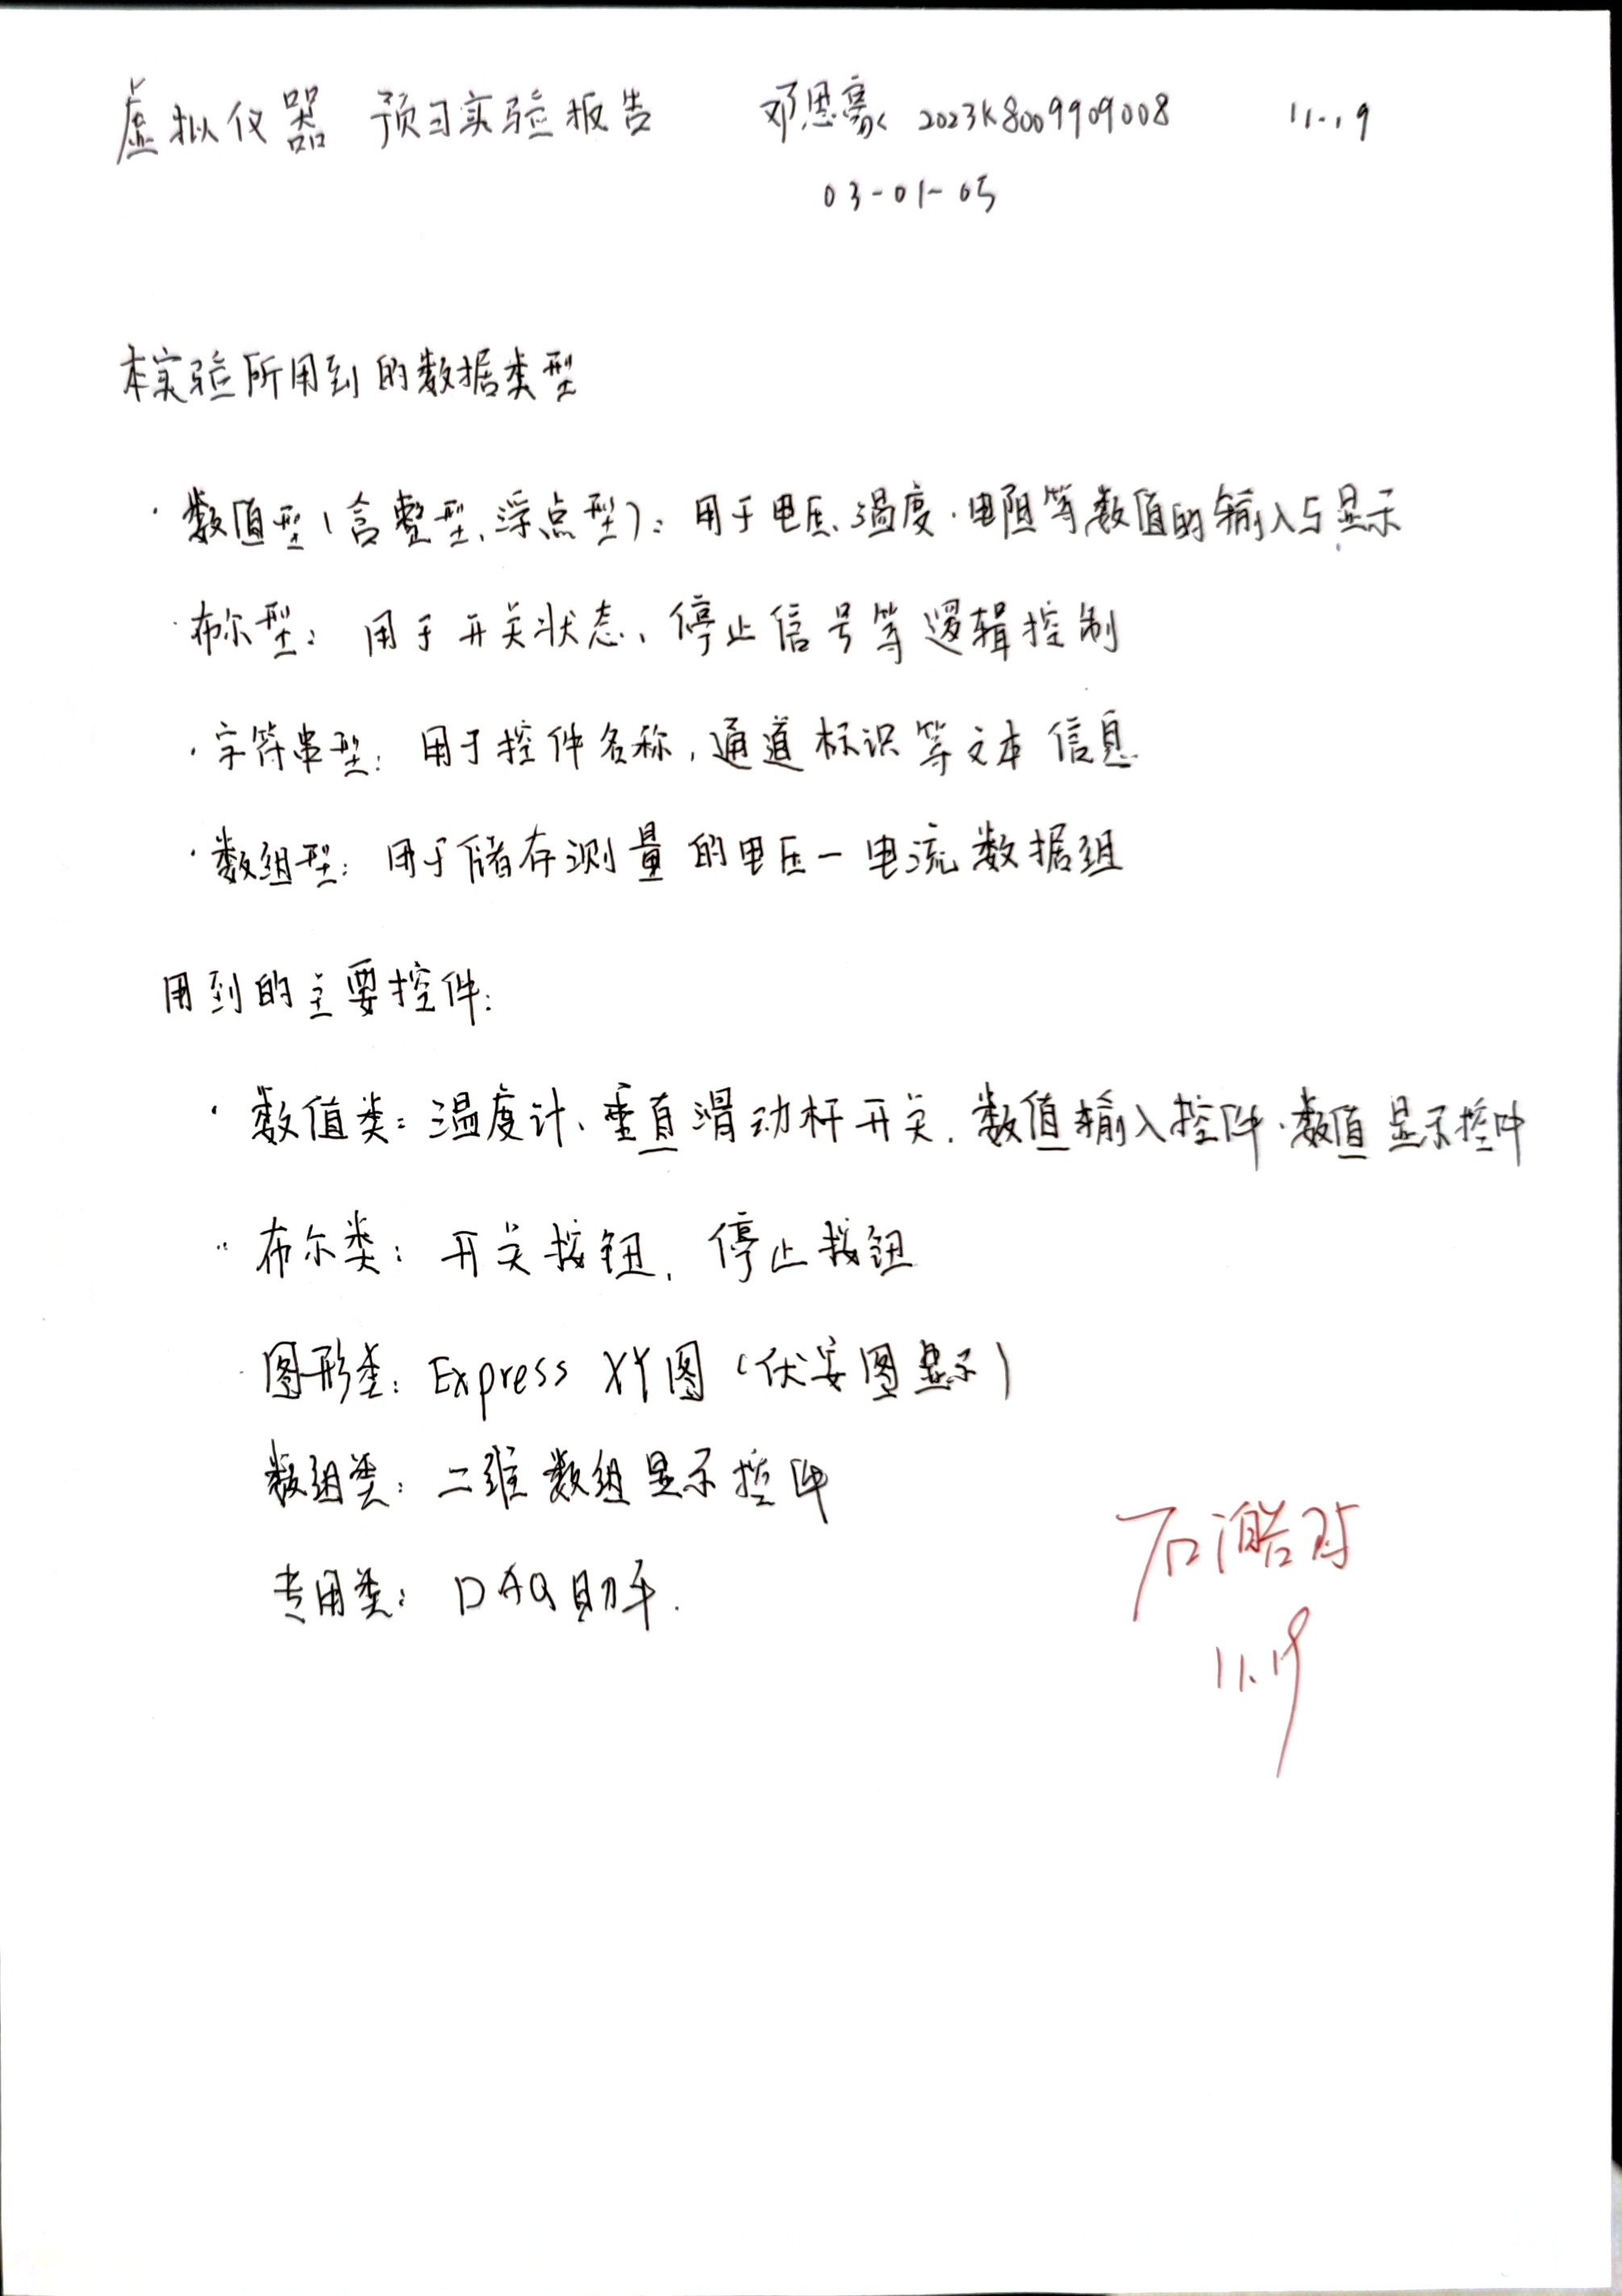
\includegraphics[width=0.7\textwidth]{Pre Report.jpg}
\end{figure}


\end{document}